%%%%%%%%%%%%%%%%%%%%%%%%%%%%%%%%%%%%%%%%%%%%%%%%%%%%%%%%%%%%%%%%%%%%%%%%%%%%%%%%%
% Template: Article
%
% Por: Abrantes Araújo Silva Filho
%      abrantesasf@gmail.com
%
% Citação: Se você gostou deste template, por favor ajude a divulgá-lo mantendo
%          o link para meu repositório GitHub em:
%          https://github.com/abrantesasf/LaTeX
%%%%%%%%%%%%%%%%%%%%%%%%%%%%%%%%%%%%%%%%%%%%%%%%%%%%%%%%%%%%%%%%%%%%%%%%%%%%%%%%%




%%%%%%%%%%%%%%%%%%%%%%%%%%%%%%%%%%%%%%%%%%%%%%%%%%%%%%%%%%%%%%%%%%%%%%%%%%%%%%%%%
%%% Configura o tipo de documento, papel, tamanho da fonte e informações básicas
%%% para as proriedades do PDF/DVIPS e outras propriedades do documento
\RequirePackage{ifpdf}
\ifpdf
  % Classe, língua e tamanho da fonte padrão. Outras opções a considerar:
  %   draft
  %   onecolumn (padrão) ou twocolumn (OU usar o package multicol)
  %   fleqn com ou sem leqno (alinhamento à esquerda das fórmulas e dos números)
  %   oneside (padrão para article ou report) ou twoside (padrão para book)
  \documentclass[pdftex, brazil, 12pt, twoside]{article}
\else
  % Classe, língua e tamanho da fonte padrão. Outras opções a considerar:
  %   draft
  %   onecolumn (padrão) ou twocolumn (OU usar o package multicol)
  %   fleqn com ou sem leqno (alinhamento à esquerda das fórmulas e dos números)
  %   oneside (padrão para article ou report) ou twoside (padrão para book)
  \documentclass[brazil, 12pt]{article}
\fi


%%%%%%%%%%%%%%%%%%%%%%%%%%%%%%%%%%%%%%%%%%%%%%%%%%%%%%%%%%%%%%%%%%%%%%%%%%%%%%%%%
%%% Carrega pacotes iniciais necessários para estrutura de controle e para a
%%% criação e o parse de novos comandos
\usepackage{ifthen}
\usepackage{xparse}


%%%%%%%%%%%%%%%%%%%%%%%%%%%%%%%%%%%%%%%%%%%%%%%%%%%%%%%%%%%%%%%%%%%%%%%%%%%%%%%%%
%%% Configuração do tamanho da página, margens, espaçamento entrelinhas e, se
%%% necessário, ativa a indentação dos primeiros parágrafos.
\ifpdf
  \usepackage[pdftex]{geometry}
\else
  \usepackage[dvips]{geometry}
\fi
\geometry{a4paper, left=2.6cm, right=4.0cm, top=3.0cm, bottom=3.4cm}

\usepackage{setspace}
  \singlespacing
  %\onehalfspacing
  %\doublespacing


%%%%%%%%%%%%%%%%%%%%%%%%%%%%%%%%%%%%%%%%%%%%%%%%%%%%%%%%%%%%%%%%%%%%%%%%%%%%%%%%%
%%% Configurações de cabeçalho e rodapé:
\usepackage{fancyhdr}
\setlength{\headheight}{1cm}
\setlength{\footskip}{1.5cm}
\renewcommand{\headrulewidth}{0.3pt}
\renewcommand{\footrulewidth}{0.0pt}
\pagestyle{fancy}
\renewcommand{\sectionmark}[1]{%
  \markboth{\uppercase{#1}}{}}
\renewcommand{\subsectionmark}[1]{%
  \markright{\uppercase{\thesubsection \hspace{0.1cm} #1}}{}}
\fancyhead{}
\fancyfoot{}
\newcommand{\diminuifonte}{%
    \fontsize{9pt}{9}\selectfont
}
\newcommand{\aumentafonte}{%
    \fontsize{12}{12}\selectfont
}
% Configura cabeçalho e rodapé para documentos TWOSIDE
\fancyhead[EL]{\textbf{\thepage}}
\fancyhead[EC]{}
\fancyhead[ER]{\diminuifonte \textbf{\leftmark}}
\fancyhead[OR]{\textbf{\thepage}}
\fancyhead[OC]{}
\fancyhead[OL]{\diminuifonte \textbf{\rightmark}}
\fancyfoot[EL,EC,ER,OR,OC,OL]{}
% Configura cabeçalho e rodapé para documentos ONESIDE
%\lhead{ \fancyplain{}{sup esquerdo} }
%\chead{ \fancyplain{}{sup centro} }
%\rhead{ \fancyplain{}{\thesection} }
%\lfoot{ \fancyplain{}{inf esquerdo} }
%\cfoot{ \fancyplain{}{inf centro} }
%\rfoot{ \fancyplain{}{\thepage} }




%%%%%%%%%%%%%%%%%%%%%%%%%%%%%%%%%%%%%%%%%%%%%%%%%%%%%%%%%%%%%%%%%%%%%%%%%%%%%%%%%
%%% Configurações de encoding, lingua e fontes:
\usepackage[T1]{fontenc}
\usepackage[utf8]{inputenc}
\usepackage{babel}

% Altera a fonte padrão do documento (nem todas funcionam em modo math):
%   phv = Helvetica
%   ptm = Times
%   ppl = Palatino
%   pbk = bookman
%   pag = AdobeAvantGarde
%   pnc = Adobe NewCenturySchoolBook
\renewcommand{\familydefault}{ppl}


%%%%%%%%%%%%%%%%%%%%%%%%%%%%%%%%%%%%%%%%%%%%%%%%%%%%%%%%%%%%%%%%%%%%%%%%%%%%%%%%%
%%% Carrega pacotes para referências cruzadas, citações dentro do documento,
%%% links para internet e outros.Configura algumas opções.
%%% Não altere a ordem de carregamento dos packages.
\usepackage{varioref}
\ifpdf
  \usepackage[pdftex]{hyperref}
    \hypersetup{
      % Informações variáveis em cada documento (MUDE AQUI!):
      pdftitle={Calculus 1A: Differentiation},
      pdfauthor={MITx on EdX},
      pdfsubject={MITx 18.01.1x on EdX --- Calculus 1A: Differentiation},
      pdfkeywords={calculus, derivative},
      pdfinfo={
        CreationDate={}, % Ex.: D:AAAAMMDDHH24MISS
        ModDate={}       % Ex.: D:AAAAMMDDHH24MISS
      },
      % Coisas que você não deve alterar se não souber o que está fazendo:
      unicode=true,
      pdflang={pt-BR},
      bookmarksopen=true,
      bookmarksnumbered=true,
      bookmarksopenlevel=5,
      pdfdisplaydoctitle=true,
      pdfpagemode=UseOutlines,
      pdfstartview=FitH,
      pdfcreator={LaTeX with hyperref package},
      pdfproducer={pdfTeX},
      pdfnewwindow=true,
      colorlinks=true,
      citecolor=green,
      linkcolor=red,
      filecolor=cyan,
      urlcolor=blue
    }
\else
  \usepackage{hyperref}
\fi
\usepackage{cleveref}
\usepackage{url}


%%%%%%%%%%%%%%%%%%%%%%%%%%%%%%%%%%%%%%%%%%%%%%%%%%%%%%%%%%%%%%%%%%%%%%%%%%%%%%%%%
%%% Carrega bibliotecas de símbolos (matemáticos, físicos, etc.), fontes
%%% adicionais, e configura algumas opções
\usepackage{amsmath}
\usepackage{amssymb}
\usepackage{amsfonts}
\usepackage{siunitx}
  \sisetup{group-separator = {.}}
  \sisetup{group-digits = {false}}
  \sisetup{output-decimal-marker = {,}}
\usepackage{bm}
\usepackage{cancel}
% Altera separador decimal via comando, se necessário (prefira o siunitx):
%\mathchardef\period=\mathcode`.
%\DeclareMathSymbol{.}{\mathord}{letters}{"3B}
  

%%%%%%%%%%%%%%%%%%%%%%%%%%%%%%%%%%%%%%%%%%%%%%%%%%%%%%%%%%%%%%%%%%%%%%%%%%%%%%%%%
%%% Carrega packages relacionados à computação
\usepackage{algorithm2e}
\usepackage{algorithmicx}
\usepackage{algpseudocode}
\usepackage{listings}
  \lstset{literate=
    {á}{{\'a}}1 {é}{{\'e}}1 {í}{{\'i}}1 {ó}{{\'o}}1 {ú}{{\'u}}1
    {Á}{{\'A}}1 {É}{{\'E}}1 {Í}{{\'I}}1 {Ó}{{\'O}}1 {Ú}{{\'U}}1
    {à}{{\`a}}1 {è}{{\`e}}1 {ì}{{\`i}}1 {ò}{{\`o}}1 {ù}{{\`u}}1
    {À}{{\`A}}1 {È}{{\'E}}1 {Ì}{{\`I}}1 {Ò}{{\`O}}1 {Ù}{{\`U}}1
    {ä}{{\"a}}1 {ë}{{\"e}}1 {ï}{{\"i}}1 {ö}{{\"o}}1 {ü}{{\"u}}1
    {Ä}{{\"A}}1 {Ë}{{\"E}}1 {Ï}{{\"I}}1 {Ö}{{\"O}}1 {Ü}{{\"U}}1
    {â}{{\^a}}1 {ê}{{\^e}}1 {î}{{\^i}}1 {ô}{{\^o}}1 {û}{{\^u}}1
    {Â}{{\^A}}1 {Ê}{{\^E}}1 {Î}{{\^I}}1 {Ô}{{\^O}}1 {Û}{{\^U}}1
    {œ}{{\oe}}1 {Œ}{{\OE}}1 {æ}{{\ae}}1 {Æ}{{\AE}}1 {ß}{{\ss}}1
    {ű}{{\H{u}}}1 {Ű}{{\H{U}}}1 {ő}{{\H{o}}}1 {Ő}{{\H{O}}}1
    {ç}{{\c c}}1 {Ç}{{\c C}}1 {ø}{{\o}}1 {å}{{\r a}}1 {Å}{{\r A}}1
    {€}{{\euro}}1 {£}{{\pounds}}1 {«}{{\guillemotleft}}1
    {»}{{\guillemotright}}1 {ñ}{{\~n}}1 {Ñ}{{\~N}}1 {¿}{{?`}}1
  }
  

%%%%%%%%%%%%%%%%%%%%%%%%%%%%%%%%%%%%%%%%%%%%%%%%%%%%%%%%%%%%%%%%%%%%%%%%%%%%%%%%%
%%% Ativa suporte extendido a cores
\usepackage[svgnames]{xcolor} % Opções de cores: usenames (16), dvipsnames (64),
                              % svgnames (150) e x11names (300).


%%%%%%%%%%%%%%%%%%%%%%%%%%%%%%%%%%%%%%%%%%%%%%%%%%%%%%%%%%%%%%%%%%%%%%%%%%%%%%%%%
%%% Suporte à importação de gráficos externos
\ifpdf
  \usepackage[pdftex]{graphicx}
\else
  \usepackage[dvips]{graphicx}
\fi


%%%%%%%%%%%%%%%%%%%%%%%%%%%%%%%%%%%%%%%%%%%%%%%%%%%%%%%%%%%%%%%%%%%%%%%%%%%%%%%%%
%%% Suporte à criação de gráficos proceduralmente na LaTeX:
\usepackage{tikz}
  \usetikzlibrary{arrows,automata,backgrounds,matrix,patterns,positioning,shapes,shadows}


%%%%%%%%%%%%%%%%%%%%%%%%%%%%%%%%%%%%%%%%%%%%%%%%%%%%%%%%%%%%%%%%%%%%%%%%%%%%%%%%%
%%% Packages para tabelas
\usepackage{array}
\usepackage{longtable}
\usepackage{tabularx}
\usepackage{tabu}
\usepackage{lscape}
\usepackage{colortbl}  
\usepackage{booktabs}


%%%%%%%%%%%%%%%%%%%%%%%%%%%%%%%%%%%%%%%%%%%%%%%%%%%%%%%%%%%%%%%%%%%%%%%%%%%%%%%%%
%%% Packages ambientes de listas
\usepackage{enumitem}
\usepackage[ampersand]{easylist}


%%%%%%%%%%%%%%%%%%%%%%%%%%%%%%%%%%%%%%%%%%%%%%%%%%%%%%%%%%%%%%%%%%%%%%%%%%%%%%%%%
%%% Packages para suporte a ambientes floats, captions, etc.:
\usepackage{float}
\usepackage{wrapfig}
\usepackage{placeins}
\usepackage{caption}
\usepackage{sidecap}
\usepackage{subcaption}


%%%%%%%%%%%%%%%%%%%%%%%%%%%%%%%%%%%%%%%%%%%%%%%%%%%%%%%%%%%%%%%%%%%%%%%%%%%%%%%%%
%%% Meus comandos específicos:
% Commando para ``italizar´´ palavras em inglês (e outras línguas!):
\newcommand{\ingles}[1]{\textit{#1}}

% Commando para colocar o espaço correto entre um número e sua unidade:
\newcommand{\unidade}[2]{\ensuremath{#1\,\mathrm{#2}}}
\newcommand{\unidado}[2]{{#1}\,{#2}}

% Produz ordinal masculino ou feminino dependendo do segundo argumento:
\newcommand{\ordinal}[2]{%
#1%
\ifthenelse{\equal{a}{#2}}%
{\textordfeminine}%
{\textordmasculine}}


%%%%%%%%%%%%%%%%%%%%%%%%%%%%%%%%%%%%%%%%%%%%%%%%%%%%%%%%%%%%%%%%%%%%%%%%%%%%%%%%%
%%% Hifenização específica quando o LaTeX/Babel não conseguirem hifenizar:
\babelhyphenation{Git-Hub}
\usepackage{exsol}



%%%%%%%%%%%%%%%%%%%%%%%%%%%%%%%%%%%%%%%%%%%%%%%%%%%%%%%%%%%%%%%%%%%%%%%%%%%%%%%%%
%%%%%%%%%%%%%%%%%%%%%%%%%%%%%%%%%%%%%%%%%%%%%%%%%%%%%%%%%%%%%%%%%%%%%%%%%%%%%%%%%
%%%%%%%%%%%%%%%%%%%%%%%%%%%%%%%%%%%%%%%%%%%%%%%%%%%%%%%%%%%%%%%%%%%%%%%%%%%%%%%%%
%%%%%%%%%%%%%%%%%%%%%%%%%%%%%%%%%%%%%%%%%%%%%%%%%%%%%%%%%%%%%%%%%%%%%%%%%%%%%%%%%
%%%%%%%%%%%%%%%%%%%%%%%%%%%%%% COMEÇA O DOCUMENTO %%%%%%%%%%%%%%%%%%%%%%%%%%%%%%%
%%%%%%%%%%%%%%%%%%%%%%%%%%%%%%%%%%%%%%%%%%%%%%%%%%%%%%%%%%%%%%%%%%%%%%%%%%%%%%%%%
%%%%%%%%%%%%%%%%%%%%%%%%%%%%%%%%%%%%%%%%%%%%%%%%%%%%%%%%%%%%%%%%%%%%%%%%%%%%%%%%%
%%%%%%%%%%%%%%%%%%%%%%%%%%%%%%%%%%%%%%%%%%%%%%%%%%%%%%%%%%%%%%%%%%%%%%%%%%%%%%%%%
%%%%%%%%%%%%%%%%%%%%%%%%%%%%%%%%%%%%%%%%%%%%%%%%%%%%%%%%%%%%%%%%%%%%%%%%%%%%%%%%%
\begin{document}
\title{Calculus 1A: Differentiation}
\author{MITx 18.01.1x}
\date{2018/08/17 -- 2018/11/20}
\maketitle
\tableofcontents
\newpage


%%%%%%%%%%%%%%%%%%%%%%%%%%%%%%%%%%%%%%%%%%%%%%%%%%%%%%%%%%%%%%%%%%%%%%%%%%%%%%%%%
%%%%%%%%%%%%%%%%%%%%%%%%%%%%%%%%%%%%%%%%%%%%%%%%%%%%%%%%%%%%%%%%%%%%%%%%%%%%%%%%%
%%%%%%%%%%%%%%%%%%%%%%%%%%%%%%%%%%%%%%%%%%%%%%%%%%%%%%%%%%%%%%%%%%%%%%%%%%%%%%%%%
\section{Getting started (2018/08/17)}
\label{gs}


%%%%%%%%%%%%%%%%%%%%%%%%%%%%%%%%%%%%%%%%%%%%%%%%%%%%%%%%%%%%%%%%%%%%%%%%%%%%%%%%%
%%%%%%%%%%%%%%%%%%%%%%%%%%%%%%%%%%%%%%%%%%%%%%%%%%%%%%%%%%%%%%%%%%%%%%%%%%%%%%%%%
\subsection{Overview and logistics}
\label{gs-ol}

%%%%%%%%%%%%%%%%%%%%%%%%%%%%%%%%%%%%%%%%%%%%%%%%%%%%%%%%%%%%%%%%%%%%%%%%%%%%%%%%%
\subsubsection{Meet the course team}
\label{gs-ol-team}

\paragraph{Professor David Jerison}
David Jerison received his Ph.D.\ from Princeton University in 1980, and joined the mathematics faculty at MIT in 1981. In 1985, he received an A.P.\ Sloan Foundation Fellowship and a Presidential Young Investigator Award. In 1999 he was elected to the American Academy of Arts and Sciences. In 2004, he was selected for a Margaret MacVicar Faculty Fellowship in recognition of his teaching. In 2012, the American Mathematical Society awarded him and his collaborator Jack Lee the Bergman Prize in Complex Analysis.

\begin{figure}[H]
  \begin{center}
    \caption{Professor David Jerison}
    \label{fig:david-jerison}
    \fbox{
\includegraphics[scale=0.7]{imagens/jerison.jpg}}
    %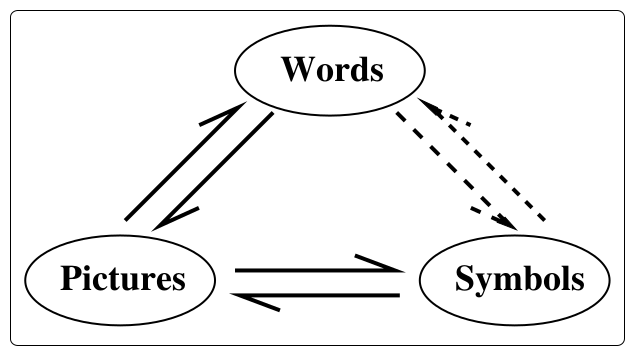
\includegraphics[scale=0.4]{imagens/palavras-imagens-simbolos.png}
    %
    %\footnotesize{Fonte:}
  \end{center}
\end{figure}

Professor Jerison's research focuses on PDEs and Fourier Analysis. He has taught single variable calculus, multivariable calculus, and differential equations at MIT several times each.

\paragraph{Professor Gigliola Staffilan}
Gigliola Staffilani is the Abby Rockefeller Mauzé Professor of Mathematics since 2007. She received her Ph.D.\ from the University of Chicago in 1995. Following faculty appointments at Stanford, Princeton, and Brown, she joined the MIT mathematics faculty in 2002. She received both a teaching award and a research fellowship while at Stanford. She received a Sloan Foundation Fellowship in 2000. In 2014 she was elected to the American Academy of Arts and Sciences.

\begin{figure}[H]
  \begin{center}
    \caption{Professor Gigliola Staffilani}
    \label{fig:gigliola}
    \fbox{
\includegraphics[scale=0.7]{imagens/staffilani.jpg}}
    %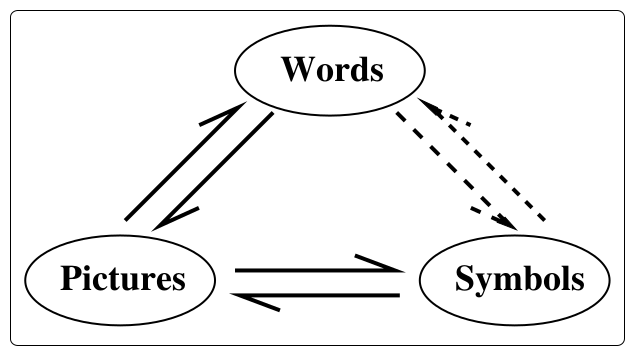
\includegraphics[scale=0.4]{imagens/palavras-imagens-simbolos.png}
    %
    %\footnotesize{Fonte:}
  \end{center}
\end{figure}

Professor Staffilani is an analyst, with a concentration on dispersive nonlinear PDEs. She has taught multivariable calculus several times at MIT, as well as differential equations.

\paragraph{Instructor Jen French}
Jen French is an MITx Digital Learning Scientist in the MIT math department. She earned her Ph.D.\ in mathematics from MIT in 2010, with specialization in Algebraic Topology. After teaching after school math for elementary aged students and working with the Teaching and Learning Lab at MIT developing interdisciplinary curricular videos tying foundational concepts in math and science to engineering design themes, she joined MITx in 2013. She has developed videos, visual interactives, and problems providing immediate feedback using the edX platform residentially in the MIT math department to aid student learning. She has developed the calculus series (3 courses) and differential equations series (5 courses) available here on edX.

\begin{figure}[H]
  \begin{center}
    \caption{Instructor Jen French }
    \label{fig:jen}
    \fbox{
\includegraphics[scale=0.7]{imagens/french.jpg}}
    %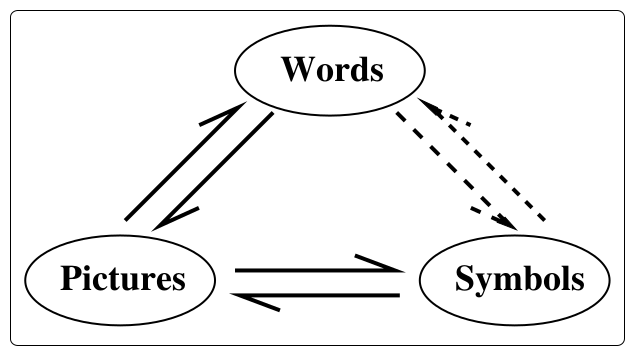
\includegraphics[scale=0.4]{imagens/palavras-imagens-simbolos.png}
    %
    %\footnotesize{Fonte:}
  \end{center}
\end{figure}

\paragraph{Instructor Stephen Wang}
Stephen Wang earned a Ph.D.\ in mathematics from the University of Chicago in 2006, where he specialized in geometry. He has earned teaching awards from both Chicago and Harvard University, and has also been a faculty member at Haverford College and Bucknell University before jumping on board the calculus team at MIT. In fall 2015 he joined the Rice University mathematics faculty.

\begin{figure}[H]
  \begin{center}
    \caption{Instructor Stephen Wang}
    \label{fig:wang}
    \fbox{
\includegraphics[scale=0.7]{imagens/wang.jpg}}
  \end{center}
\end{figure}

\paragraph{Special thanks to \ldots}
Huge thanks to Prof. Arthur Mattuck for starting it all. Big thanks to Timothy Hall for asking David Jerison the question, how do ziplines behave mathematically. We also thank David Custer and Susan Ruff who helped with real life ziplines and shared MIT student experiments on ziplines.

Ed Tech Developers:
\begin{itemize}[noitemsep]
\item J.\ M.\ Claus
\item Brian French
\item Eric Heubel
\item Haynes Miller
\item Martin Segado
\end{itemize}

MIT Undergrads:
\begin{itemize}[noitemsep]
\item Phillip Ai
\item Emanuele Ceccarelli
\item Peter Haine
\item Peter Kleinhenz
\item Mohammed Kane
\end{itemize}

MIT PhD Students:
\begin{itemize}[noitemsep]
\item Tudor Cristea-Platon
\item Kristin Kurianski
\item Lucas Tambasco
\end{itemize}

MITx Video Team:
\begin{itemize}[noitemsep]
\item Brittany Bellamy
\item Chris Boebel
\item Kenny Caudill
\item Tsinu Heramo
\item Jess Kloss
\item Douglass McLean
\item Lana Scott
\item Catilin Stier
\end{itemize}

MITx Support Staff:
\begin{itemize}[noitemsep]
\item Kyle Boots
\item Brad K.\ Goodman
\end{itemize}

\fbox{\begin{minipage}{10cm}This course was funded in part by:\ \\
Class of 1960 Alumni Funds\ \\
2014--2015 Alumni Class Funds Grant\ \\
Wertheimer Fund\end{minipage}}

%%%%%%%%%%%%%%%%%%%%%%%%%%%%%%%%%%%%%%%%%%%%%%%%%%%%%%%%%%%%%%%%%%%%%%%%%%%%%%%%%
\subsubsection{Course description}
\label{gs-ol-description}

Discover the derivative --- what it is, how to compute it, and when to apply it in solving real world problems. Part 1 of 3.

How does the final velocity on a zip line change when the starting point is raised or lowered by a matter of centimeters? What is the accuracy of a GPS position measurement? How fast should an airplane travel to minimize fuel consumption? The answers to all of these questions involve the derivative.

But what is the derivative? You will learn its mathematical notation, physical meaning, geometric interpretation, and be able to move fluently between these representations of the derivative. You will discover how to differentiate any function you can think up, and develop a powerful intuition to be able to sketch the graph of many functions. You will make linear and quadratic approximations of functions to simplify computations and gain intuition for system behavior. You will learn to maximize and minimize functions to optimize properties like cost, efficiency, energy, and power.

This course, in combination with \emph{18.01.2x Calculus 1B: Integration}, covers the AP Calculus AB curriculum.

This course, in combination with \emph{18.01.2x Calculus 1B: Integration} and \emph{18.01.3x Calculus 1C: Coordinate Systems and Infinite Series}, covers the AP Calculus BC curriculum.

If you intend to take an AP exam, we strongly suggest that you familiarize yourself with the AP exam to prepare for it.

%%%%%%%%%%%%%%%%%%%%%%%%%%%%%%%%%%%%%%%%%%%%%%%%%%%%%%%%%%%%%%%%%%%%%%%%%%%%%%%%%
\subsubsection{The making of this course}
\label{gs-ol-making}

This course was created using latex2edX, a free tool developed at MIT for creating content for edX written in \LaTeX. \LaTeX\ is a typesetting language that is fantastic for writing math! Occasionally, the equations you see in the webpage (which are rendered in mathjax) do not load appropriately. Our apologies. The easiest fix is to simply reload the page. Another solution is to change browsers. (Firefox seems to render mathjax less reliably than Chrome or Safari. However, frequent changes to edX will cause disruptions in our content.)

Note edX is not supported on tablet devices. That said, users report that 95\% of the problems can be done on a tablet device, but if weird errors are creeping in (especially with formula input type problems) you may try switching to a laptop or desktop computer.

\begin{figure}[H]
  \begin{center}
    %\caption{}
    \label{fig:latex2edx}
    \fbox{
\includegraphics[scale=0.7]{imagens/latex2edx.png}}
  \end{center}
\end{figure}
 
%%%%%%%%%%%%%%%%%%%%%%%%%%%%%%%%%%%%%%%%%%%%%%%%%%%%%%%%%%%%%%%%%%%%%%%%%%%%%%%%%
\subsubsection{How to succeed}
\label{gs-ol-succeed}

\paragraph{Prerequisites}
This course has a global audience with students from a wide variety of backgrounds. To succeed in this course, you must have a solid foundation in

\begin{enumerate}[noitemsep]
\item Algebra
\item Geometry
\item Trigonometry
\item Exponents
\item Logarithms
\item Limits
\end{enumerate}

We know that many students may not have solid foundation in limits, so we have included an optional Unit 0 that introduces Limits. Understanding limits is essential to understand the first lecture on the definition of the derivative in Unit 1, some Homework problems on Continuity and Differentiability in Unit 1, and the first lecture on Limiting behavior and sketching functions in Unit 4.

Because we know you come from different backgrounds, we want to help you to choose the best path through this content. To aid us in this, please take the ``Choose your calculus adventure'' diagnostics. This will help you to determine if you have the skills to succeed, what skills you may need to review, and which units you may be able to skip!

\paragraph{Reference materials}
The material we provide in the Courseware contains all of the content you need for this course. However, there are many good calculus texts that have a great deal of problems and alternate explanations that may help you. Most widely used calculus texts are adequate.

There is also the free web resource \href{https://www.khanacademy.org/}{Khan Academy}.
Links to other web resources can be found on the Course Info page under the header ``Related Links''. Feel free to share other resources on the course wiki or through the discussion forum.

%%%%%%%%%%%%%%%%%%%%%%%%%%%%%%%%%%%%%%%%%%%%%%%%%%%%%%%%%%%%%%%%%%%%%%%%%%%%%%%%%
\subsubsection{Grading}
\label{gs-ol-grading}

There are 4 categories of graded problems in 18.01.1x: in-lecture Exercises, Part A Homework, Part B Homework, and the Final Exam.

\begin{itemize}
\item \textbf{Exercises:} These are the problems that are interspersed between videos in each lecture. These problems count for 20\% of your grade. These problems will be used to motivate theory, practice a concept you just learned, and review material from previous sequences that we are using. While you are graded on these problems, they are low-stakes: you have multiple attempts, and have the opportunity to look at the answer after you have submitted a correct answer or run out of attempts. This is where you will do the majority of your learning. We encourage you to make mistakes and learn from them!
\item \textbf{Part A Homework:} Each unit has 1 Part A Homework assignment, which gives you an opportunity to practice what you learned. These problems count for 10\% of your total grade. Wait until the end of the unit to attempt these problems. These problems help you identify the concepts that you have forgotten, and aid in long-term retention. These problems are mostly mechanical–asking you to practice methods, and techniques learned in each unit. Each problem typically tests knowledge from only one section in a unit. (We won't necessarily tell you which one though!)
\item \textbf{Part B Homework:} Each unit has 1 Part B Homework assignment. The part B homework counts for 25\% of your total grade. The problems on this homework combine ideas from all of the sequences in the unit. These problems are mostly in the form of word problems which ask you to apply the methods learned to new scenarios.
\item \textbf{Final:} The final exam is the culmination of your learning, and will account for 45\% of your grade. These problems cover all of the material in this course. Several of the problems follow the AP short-answer format. However, we cannot grade the justifications to your reasoning here. To prepare for the AP exam, you should take and review the solutions to sample AP exams from the AP website. 
\end{itemize}

Note: Please notice that Unit 0 is optional and the exercises and homework are intended for self study only and do not count towards your grade.

\paragraph{Certification} To earn an ID verified certificate, you must earn 60\% of the points in this course. You can see your progress towards certification by clicking on the Progress link above.


%%%%%%%%%%%%%%%%%%%%%%%%%%%%%%%%%%%%%%%%%%%%%%%%%%%%%%%%%%%%%%%%%%%%%%%%%%%%%%%%%
%%%%%%%%%%%%%%%%%%%%%%%%%%%%%%%%%%%%%%%%%%%%%%%%%%%%%%%%%%%%%%%%%%%%%%%%%%%%%%%%%
\subsection{Using the EdX platform}
\label{gs-edx}

%%%%%%%%%%%%%%%%%%%%%%%%%%%%%%%%%%%%%%%%%%%%%%%%%%%%%%%%%%%%%%%%%%%%%%%%%%%%%%%%%
\subsubsection{Navigating EdX}
\label{gs-edx-nav}

This course was developed at MIT and is made available to you by the edX platform.The edX platform is a platform for learning! It allows people from around the world to access content for free, based on their own interests and background.

If you have never taken a course on edX, please take the short 1 hour course
\href{https://www.edx.org/course/demox-edx-demox-1-0}{DemoX} to familiarize yourself with the platform and its capabilities.

In this course, we have the following top-level resources:

\begin{itemize}[noitemsep]
\item \textbf{Course:} This is the graded content of this course, as well as all learning materials.
\item \textbf{Calendar:} All of the due dates are in UTC, and are available in the google calendar,
  which you can download into your own calendar so that you can have these due dates available in your own time zone.
\item \textbf{Discussion:} This is a link to the full discussion forum. For specific discussions
  related to a problem or video, link through the discussion forum link at the bottom of each page.
  (See the discussion at the bottom of this page for help with these problems.)
\item \textbf{Progress:} Use this tab to see how your are progressing through the content!
\end{itemize}

\textbf{Course} is where you will spend most of your time. This is where we put the content and assessments for your learning. Everything else is a resource to support your learning.

%%%%%%%%%%%%%%%%%%%%%%%%%%%%%%%%%%%%%%%%%%%%%%%%%%%%%%%%%%%%%%%%%%%%%%%%%%%%%%%%%
\subsubsection{Example problem types}
\label{gs-edx-example}

Take a moment to familiarize yourself with the main problem types we use in this course.

\paragraph{Checking and submitting an answer:}
The edX platform is able to check your answers and give you immediate feedback. When you ``check'' a problem, it is automatically submitted for grading purposes. Depending on the type of the problem you may have access to the ``show answer'' button. In the lecture exercises as well as the part A and part B Homework assignments, this option to show the answer will appear only after the due date has passed, you have run out of problem attempts, or you have already submitted the correct answer. You will never get detailed solutions to the final exam.
Example: \emph{This problem has unlimited attempts. If you get an answer wrong, you can simply try again until you get it right. How many weeks will this course be?}

\paragraph{Resetting a Problem:}
Some problems involve randomized parameters, or other elements that you may wish to reset to the original configuration. Here is an example where the variables and are randomized. After one attempt, you can click reset to see the values change!
Example: \emph{Let $x_1 = 5$ and $x_2 = 65$. Enter the numeric value of in the answer box below.}

\paragraph{Limited Number of Attempts 1:}
Most of the time, you will have a limited number of times that you can attempt a problem. To save an answer and keep it there until you come back, use the save button.
Example: \emph{How much does it cost to take an edX course?}

\paragraph{Limited Number of Attempts 2:}
Multiple choice problems will almost always have between 1 and 3 attempts.
Example: \emph{Which choice is correct?}

\paragraph{Formula Entry Problems:}
This is a math class, which means we are going to be using formulas. And sometimes, we want you to find these formulas. There are some rules for entering formulas into the text entry box (which follows rules for ASCII math). Use:

\begin{itemize}[noitemsep]
\item $+$ to denote addition; e.g. $2+3$
\item $-$ to denote subtraction; e.g. $x-1$
\item $*$ to denote multiplication; e.g. $2*x$
\item $\wedge$ to denote exponentiation; e.g. $x \wedge 2$ for $x^2$
\item / to denote division; e.g. $7/x$ for $\frac{7}{x}$
\item ``pi'' for the mathematical constant $\pi$
\item ``e'' for the mathematical constant $e$
\item sqrt(x), sin(x), cos(x), ln(x), arccos(x), etc. for the known functions $\sqrt{x}$, $\sin{x}$, $\cos{x}$, $\ln{x}$, etc. Note that parentheses are required.
\item Use parentheses ( ) to specify order of operations.
\end{itemize}

Each formula entry box will have a Formula Input Help button below the answer button, where you can find these facts about how to enter formulas. (See the button below.) Example: \emph{enter the function $2e^{x-1} + \sqrt{y}$ using the rules above. (Type 2 * e \textasciicircum (x-1) + sqrt(y) into the answer box.)}

\paragraph{Drag and Drop Problems:}
Example: \emph{Drag and drop the elements to create the quadratic formula}. 
Use the arrows on the horizontal bar to see more options to drag into the formula.

\paragraph{Sketch Input Problems:}
We created this sketch input problem type because being able to sketch functions to reason through problems is a big part of applying calculus as a problem-solving tool. Example: \emph{Try drawing a smiley face. The mouth should lie below the x-axis, and the place an eye at the points and $(-1, 2)$ and $(1, 2)$}


%%%%%%%%%%%%%%%%%%%%%%%%%%%%%%%%%%%%%%%%%%%%%%%%%%%%%%%%%%%%%%%%%%%%%%%%%%%%%%%%%
%%%%%%%%%%%%%%%%%%%%%%%%%%%%%%%%%%%%%%%%%%%%%%%%%%%%%%%%%%%%%%%%%%%%%%%%%%%%%%%%%
\subsection{Using the forum}
\label{gs-forum}

%%%%%%%%%%%%%%%%%%%%%%%%%%%%%%%%%%%%%%%%%%%%%%%%%%%%%%%%%%%%%%%%%%%%%%%%%%%%%%%%%
\subsubsection{Discussion forum}
\label{gs-forum-forum}

The discussion forum is the tool for connecting with the community of online learners in this course. Use the forum to ask questions, seek clarifications, report bugs, start or respond to topical discussions.

On most pages, there is a link at the bottom, which says ``show discussion''. Clicking this link will show the discussion forum associated with the videos and problems on that page.

\paragraph{``Netiquette'': What to do}

\begin{itemize}[noitemsep]
\item \textbf{Be polite.} Make sure that your posts are respectful of the other students and staff in the course.
\item Use the search button. Search for similar forum posts \textbf{before you post} using the magnifying glass icon. Many of your classmates will have the same question that you do! If you perform a search first, you may find the question and answer without needing to post yourself. This helps us keep the forum organized and useful!
\item Reply to existing discussions when you see someone with the same question. This helps to organize responses.
\item Use a descriptive and specific title to your post. This will attract the attention of TAs and classmates who can answer your question.
\item Be very specific about where you need help. Are you stuck on a particular part of a problem? Are you confused by a particular concept? What have you done so far?
\item Actively up-vote other posts, and other students will up-vote yours! The more up-votes your post has, the more likely they are to be seen.
\end{itemize}

\paragraph{``Netiquette'': What not to do}
Follow common writing practices for online communication:

\begin{itemize}[noitemsep]
\item Avoid TYPING IN ALL CAPS. Some people read this as shouting, even if that is not your intention.
\item Avoid \textbf{typing in bold}. Some people read this as shouting, even if that is not your intention.
\item Avoid unnecessary symbols, abbreviated words, texting shorthand, and replacing words with numbers (e.g. Pls don't rplce wrds w/\#s).
\item Avoid repeating letters or reeeeepeeaattinggggg chaaracterrrss.
\item Avoid excessive punctuation!!!!!!!!
\end{itemize}

\paragraph{Cheating!}
We encourage you to communicate in the forum about problems, and get hints and help understanding the material from your fellow classmates and the course TAs. However:

\begin{itemize}[noitemsep]
\item Please do not post solutions to lecture problems, homework problems (part A or part B), or final exam problems. These will be removed, and the student who posted will be contacted and dealt with individually.
\item Do not post or copy solutions posted to the forum for any exercises. This is cheating.
\item Do not copy solutions from yourself. This is cheating.
\end{itemize}


%%%%%%%%%%%%%%%%%%%%%%%%%%%%%%%%%%%%%%%%%%%%%%%%%%%%%%%%%%%%%%%%%%%%%%%%%%%%%%%%%
%%%%%%%%%%%%%%%%%%%%%%%%%%%%%%%%%%%%%%%%%%%%%%%%%%%%%%%%%%%%%%%%%%%%%%%%%%%%%%%%%
\subsection{Choose your calculus adventure}
\label{gs-adventure}

%%%%%%%%%%%%%%%%%%%%%%%%%%%%%%%%%%%%%%%%%%%%%%%%%%%%%%%%%%%%%%%%%%%%%%%%%%%%%%%%%
\subsubsection{Choose your own calculus adventure}
\label{gs-adventure-choose}

You are interested in learning calculus, but we don't know very much about you or what you already know. So to help you learn best, please take the following diagnostics. These diagnostics will help you choose a path through the content that makes the most sense for you.

We want you to succeed, so make sure that you have the basic precalculus skills so you won't be frustrated! The first 4 pages test your readiness for this calculus class. If you aren't ready yet, don't worry, you can take this course later.

Some of you may already know a lot of calculus. To help you get started in the right place, we have further diagnostics. On pages 5 and 6, you can take the limits and derivatives diagnostics. We encourage you to take a look at these even if you don't know any calculus yet. But don't worry; we designed this course for people with varying backgrounds, including those with no calculus experience.

%%%%%%%%%%%%%%%%%%%%%%%%%%%%%%%%%%%%%%%%%%%%%%%%%%%%%%%%%%%%%%%%%%%%%%%%%%%%%%%%%
\subsubsection{Algebra Problems}
\label{gs-adventure-algebra}

\paragraph{A1:} What is the slope of the line through the points $(3, -5)$ and $(1, -1)$?

\paragraph{A2:} The lines $3x + 27 = 7$ and $x - 3y = 6$ intersect in a point with what coordinates?

\paragraph{A3:} Which expression is equivalent to $\displaystyle \left(\frac{1}{x}+\frac{1}{y}\right)^{-1}$?

\paragraph{A4:} List all possible solutions to the equation $x^3 - x^2 - 2x = 0$ (Use decimals only, not fractions,
and separate answers with commas.)

\paragraph{A5:} A $0.25$ mL sample of water drawn from a $5$ liter flask contains $1.25 \times 10^8$ bacteria. Give the
approximate number of bacteria in the flask, expressing your answer in scientific notation.
(Scientific Notation: find a real number $a$
between $1$ and $10$, and an integer $n$, such that $x = a \times 10^n$.)

\paragraph{A6:} For what value of the constant $a$ will the system of linear equations have no solution?

\begin{equation}
  \begin{split}
    6x - 5y &= 3\\
    3x + ay &= 1
  \end{split}
\end{equation}

\paragraph{A7:} Find the value of the constant $a$ for which the polynomial $x^3 + ax^2 -1$ will have $-1$ as a zero.

\paragraph{A8:} If $\displaystyle a_n = \frac{x^n}{2^nn!}$, find $\displaystyle \frac{a_{n+1}}{a_n}$.
\ \\

If you score $0.6$ or above, you have a good grasp of algebraic manipulations, and can do them accurately enough to succeed in this class!
Otherwise, this course will be very difficult for you. We recommend taking an algebra and/or trigonometry class to solidify your familiarity and accuracy before attempting this course.

%%%%%%%%%%%%%%%%%%%%%%%%%%%%%%%%%%%%%%%%%%%%%%%%%%%%%%%%%%%%%%%%%%%%%%%%%%%%%%%%%
\subsubsection{Geometry}
\label{gs-adventure-geometry}

\paragraph{G1:} A bed that is $4$ feet wide must enter through a door along the $8$ foot wall of a $8$ by $20$ foot room.
What is the largest length of a bed that can be rotated to fit into the position shown by the dotted lines against the back wall?

\begin{figure}[H]
  \begin{center}
    %\caption{}
    \label{fig:adv-g1}
    \fbox{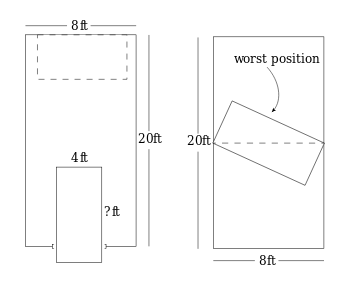
\includegraphics[scale=0.5]{imagens/adventure_g1.png}}
  \end{center}
\end{figure}

\paragraph{G2:} The four-sided solid shown is the part of the solid sphere (of radius 2, centered at the origin) in the first octant. Find its total surface area.

\begin{figure}[H]
  \begin{center}
    %\caption{}
    \label{fig:adv-g2}
    \fbox{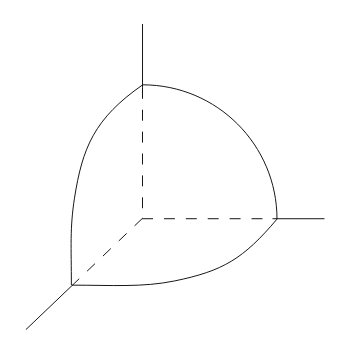
\includegraphics[scale=0.5]{imagens/adventure_g2.png}}
  \end{center}
\end{figure}

\paragraph{G3:} To estimate the height of a skyscraper 1km in the distance, Jenny finds that if her friend Steve stands 2.5 meters away, the top of his head just lines up with the top of the building. Steve is 2 meters tall, and Jenny's eye is 1.5 meters from the ground. How high is the building? (The dotted lines may help you.)

\begin{figure}[H]
  \begin{center}
    %\caption{}
    \label{fig:adv-g3}
    \fbox{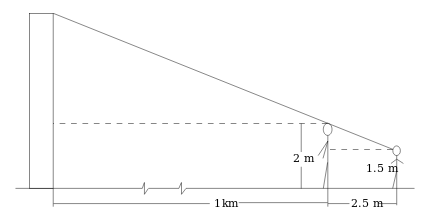
\includegraphics[scale=0.5]{imagens/adventure_g3.png}}
  \end{center}
\end{figure}

%%%%%%%%%%%%%%%%%%%%%%%%%%%%%%%%%%%%%%%%%%%%%%%%%%%%%%%%%%%%%%%%%%%%%%%%%%%%%%%%%
\subsubsection{Trigonometry}
\label{gs-adventure-trigonometry}

\paragraph{T1:} In the given right triangle, what is $\tan{y}$?

\begin{figure}[H]
  \begin{center}
    %\caption{}
    \label{fig:adv-t1}
    \fbox{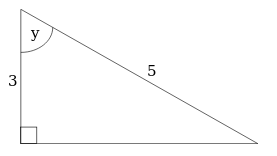
\includegraphics[scale=0.5]{imagens/adventure_t1.png}}
  \end{center}
\end{figure}

\paragraph{T2:} A horse runs counterclockwise (anticlockwise) around the circular track of radius 400m at a constant speed, starting at the marked point. It completes one lap in three minutes. What is its coordinate after one minute? (If needed, you can use ``pi'' for $\pi$, and sqrt(5) for $\sqrt{5}$.)

\begin{figure}[H]
  \begin{center}
    %\caption{}
    \label{fig:adv-t2}
    \fbox{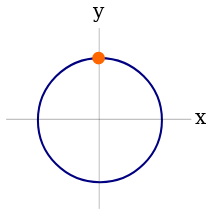
\includegraphics[scale=0.5]{imagens/adventure_t2.png}}
  \end{center}
\end{figure}

\paragraph{T3:} Find the smallest positive solution to the equation $\sin{2x} = \frac{1}{2}$; here $x$ is in radians.
(If needed, you can use ``pi'' for $\pi$, and sqrt(5) for $\sqrt{5}$. You can enter fractions using the forward slash
/ ; e.g. pi/2 for $\frac{\pi}{2}$.)

\paragraph{T4:} A line with slope 1/2 makes an acute angle $\theta$ with the axis. What is $\sin{\theta}$?
(If needed, you can use pi for $\pi$, and sqrt(5) for $\sqrt{5}$. You may enter your answer as a decimal number.)

\paragraph{T5:} By using the trigonometric identity $\cos{2x} = \cos^2{x} - \sin^2{x}$, and other identities,
find the \textbf{positive} expression for $\sin{\left(\frac{A}{2}\right)}$ in terms of $\cos{A}$.

\paragraph{T6:} The graph below represents which of these functions?

\begin{figure}[H]
  \begin{center}
    %\caption{}
    \label{fig:adv-t3}
    \fbox{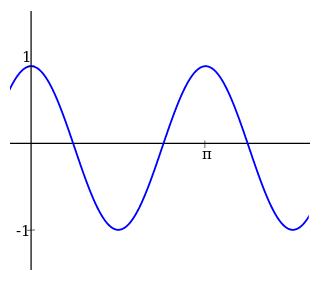
\includegraphics[scale=0.5]{imagens/adventure_t3.png}}
  \end{center}
\end{figure}

\begin{itemize}[noitemsep]
\item[$\square$] $\sin{x}$
\item[$\square$] $\cos{x}$
\item[$\square$] $\sin{(x/2)}$
\item[$\square$] $\cos{(x/2)}$
\item[$\square$] $\sin{2x}$
\item[$\square$] $\cos{2x}$
\end{itemize}

If you got a 0.6 or above, you have the foundational trigonometry understanding to succeed in this course.
Otherwise, you will need to study trigonometry concurrent with this course in order to succeed!

%%%%%%%%%%%%%%%%%%%%%%%%%%%%%%%%%%%%%%%%%%%%%%%%%%%%%%%%%%%%%%%%%%%%%%%%%%%%%%%%%
\subsubsection{Logarithms and exponentials}
\label{gs-adventure-log}

\paragraph{E1:} If $\log_{10}{a}=4.2$ and $\log_{10}{b} = 0.5$, what is $\log_{10}{ab}$?

\paragraph{E2:} If $2^a = \frac{\sqrt{8}}{4^3}$, what is $a$?

\paragraph{E3:} Which of the following is equal to $\sqrt{\frac{x^{16}(1 + x^2)}{9}}$?

\begin{itemize}
\item[$\square$] $\frac{x^4(1+x)}{3}$
\item[$\square$] $\frac{x^8(1+3)}{3}$
\item[$\square$] $\frac{x^4(1+x^2)^{0.5}}{3}$
\item[$\square$] $\frac{x^8(1+x^2)^{0.5}}{3}$
\item[$\square$] $\frac{x^4(1+x^2)}{3}$
\item[$\square$] $\frac{x^8(1+x^2)}{3}$
\item[$\square$] None of the above
\end{itemize}

\paragraph{E4:} Solve for $x$: $\log_{10}\left[(x+1)^2\right] = 2$. (Enter your answer as a list of $x$-values, separated by commas.)

\paragraph{E5:} A pot of water (at sea level) is boiling; the heat is turned off at time $t=0$, and $2$ minutes later the water temperature has fallen to $80$ºC. If the temperature $T$ (in ºC) is expressed in terms of time $t$ (in minutes) by the law

\begin{equation}
  T = Ae^{-kt}
\end{equation}
\noindent
find the values of the constants $A$ and $k$.

If you got a 0.7 or higher, congratulations! You have an excellent understanding of logarithms and exponents! Good work.
You can still succeed in this course if you got a 0.7 or lower, but we strongly recommend that you review logarithms and exponents before you get to the end of Unit 2: Differentiation where logarithms and exponents begin to take on a prominent role in the course.

%%%%%%%%%%%%%%%%%%%%%%%%%%%%%%%%%%%%%%%%%%%%%%%%%%%%%%%%%%%%%%%%%%%%%%%%%%%%%%%%%
\subsubsection{Limits diagnostic}
\label{gs-adventure-limits}

You will NOT see which problems you get correct and incorrect. Sorry if this is frustrating. We will be using these problems to assess whether or not our content teaches you about limits.

\paragraph{L1:} What is $\displaystyle \lim_{x\to\infty} \frac{x^2-4}{2 + x - 4x^2}$?

\begin{itemize}
\item[$\square$] $-2$
\item[$\square$] $-\frac{1}{4}$
\item[$\square$] $\frac{1}{2}$
\item[$\square$] $1$
\item[$\square$] The limit does not exist.
\end{itemize}

\paragraph{L2:} The graph of a function $f$ is shown below. If the limit as $x\to\infty$ exists and $f$ is not continuous at $b$, then $b=$?

\begin{figure}[H]
  \begin{center}
    %\caption{}
    \label{fig:adv-l2}
    \fbox{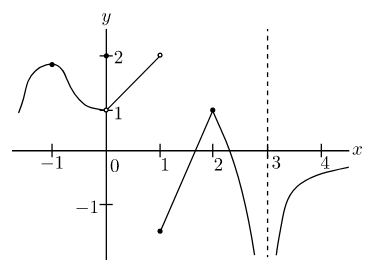
\includegraphics[scale=0.5]{imagens/adventure_l2.png}}
  \end{center}
\end{figure}

\begin{itemize}[noitemsep]
\item[$\square$] $-1$
\item[$\square$] $0$
\item[$\square$] $1$
\item[$\square$] $2$
\item[$\square$] $3$
\end{itemize}

\paragraph{L3:} What is $\displaystyle \lim_{x \to 3} \frac{6/x - 2}{3 -4x + x^2}$? (If the limit does not exist, enter DNE.)

\paragraph{L4:} Which of the following functions have a removable discontinuity at $x=2$?

\begin{itemize}
\item[$\square$] $f(x) = \frac{x^2 - x - 2}{x - 2}$
\item[$\square$] $f(x) = \frac{1}{(x-2)^2}$
\item[$\square$] $f(x) = \begin{cases}
      \frac{x^2 - x - 2}{x-2} & x \ne 2\\
      3                       & x = 2
    \end{cases}$
\item[$\square$] $f(x) = \begin{cases}
      x^3 - 1 & x > 2\\
      -x^2    & x \le 2
    \end{cases}$ 
\end{itemize}

\paragraph{L5:} Identify the left-hand limit $\displaystyle \lim_{x \to -1^-} f(x)$ based on the graph of shown below.

\begin{figure}[H]
  \begin{center}
    %\caption{}
    \label{fig:adv-l5}
    \fbox{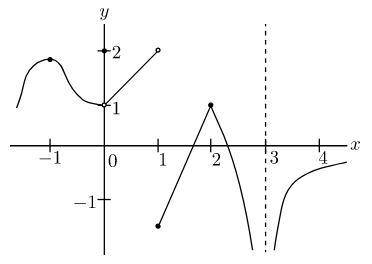
\includegraphics[scale=0.5]{imagens/adventure_l5.png}}
  \end{center}
\end{figure}

\begin{itemize}[noitemsep]
\item[$\square$] $2$
\item[$\square$] $1$
\item[$\square$] $0$
\item[$\square$] $-1$
\item[$\square$] $-1.5$
\item[$\square$] Does not exist.
\end{itemize}

\paragraph{L6:} Identify the right-handed limit $\displaystyle \lim_{x \to -1^+} \frac{x^2 -1}{|x+1|}$.
(Enter DNE if the limit does not exist.)

\begin{itemize}[noitemsep]
\item If you got 0.65 or above, you have a good handle on limits. Move on to Unit 1.
  You can go back to Unit 0 at any time to fill any gaps in your understanding of limits.
\item If you got between .35--.65 points, we recommend that you start by doing the in-lecture
  problems in Unit 0. You may be able to skip the video tutorials.
\item Otherwise, start with Unit 0!
\end{itemize}

%%%%%%%%%%%%%%%%%%%%%%%%%%%%%%%%%%%%%%%%%%%%%%%%%%%%%%%%%%%%%%%%%%%%%%%%%%%%%%%%%
\subsubsection{Derivatives diagnostic}
\label{gs-adventure-derivative}

You will not see which problems you get correct and incorrect. Sorry if this is frustrating. We will be using these problems to assess whether or not our content teaches you about derivatives.

\paragraph{C1:} What is $\displaystyle \lim_{h \to 0} \frac{\cos{(\pi/6 + h)}-\cos{(\pi/6)}}{h}$? 
(Enter the answer as a decimal. If the limit does not exist, enter DNE.)

\paragraph{C2:} At which of the five points on the graph are $\frac{dy}{dx}$ and $\frac{d^2y}{dx^2}$ both negative?

\begin{figure}[H]
  \begin{center}
    %\caption{}
    \label{fig:adv-c2}
    \fbox{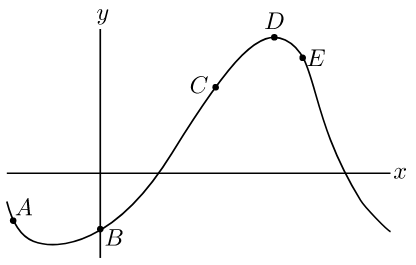
\includegraphics[scale=0.5]{imagens/adventure_c2.png}}
  \end{center}
\end{figure}

\paragraph{C3:} What is the average rate of change of the function $f(x) = x^4 - 5x$ between $x=0$ and $x=3$?

\paragraph{C4:} The position of a particle moving along a line is $p(t) = 2t^3 -24 t^2 +90t + 7$ for $t \ge 0$.
For what values of $t$ is the speed of the particle increasing?

\begin{itemize}[noitemsep]
\item[$\square$] $3 < t < 4$ only
\item[$\square$] $t > 4$ only
\item[$\square$] $t > 5$ only
\item[$\square$] $0 < t < 3$ and $t > 5$
\item[$\square$] $3 < t < 4$ and $t > 5$
\end{itemize}

\paragraph{C5:} Evaluate the limit $\lim_{x \to \infty} \frac{\ln{x}}{x^2}$:

\begin{itemize}[noitemsep]
\item[$\square$] $0$
\item[$\square$] $1$
\item[$\square$] $-1$
\item[$\square$] $\infty$
\item[$\square$] $-\infty$
\end{itemize}

\paragraph{C6:} If $f$ is differentiable at $x=a$, which of the following must be true? Choose all of the following that must be true.

\begin{itemize}[noitemsep]
\item[$\square$] $f$ is continuous at $x=a$.
\item[$\square$] $\lim_{x \to a} f(x)$ exists.
\item[$\square$] $\lim_{x \to a} \frac{f(x) - f(a)}{x-a}$ exists.
\item[$\square$] $f'(a)$ is defined.
\item[$\square$] $f''(a)$ is defined.
\end{itemize}

\paragraph{C7:} Let $f(x)=x^3 + 5x^2 -7x -1$. What is $f'(1)$?

\paragraph{C8:} Let $g(x) = x^2e^x$. What is $g'(1)$?

\paragraph{C9:} Suppose that $f(x) = g(5x)$ for all $x$, and that both functions
are differentiable. Which of the following is necessarily true?

\begin{itemize}[noitemsep]
\item[$\square$] $f'(1) = g'(1)$
\item[$\square$] $f'(5) = g'(1)$
\item[$\square$] $f'(1) = g'(5)$
\item[$\square$] $5f'(1) = g'(1)$
\item[$\square$] $5f'(1) = g'(5)$
\item[$\square$] $f'(1) = 5g'(1)$
\item[$\square$] $f'(1) = 5g'(5)$
\item[$\square$] None of the above.
\end{itemize}

\paragraph{C10:} Let $\displaystyle f(x) = \frac{\ln{(5t+1)}}{\sqrt{t+1}}$. What is $f'(0)$?

If you got 0.8 or above, you have a good handle on the derivative. There is likely no material
in Unit 0 or Unit 1 that you are not familiar with. You may choose to the the
in-lecture exercises, but may wish to skip the video tutorials. If you got less than 0.8, that is to be expected!
We assume you are here to learn about differentiation after all.


%%%%%%%%%%%%%%%%%%%%%%%%%%%%%%%%%%%%%%%%%%%%%%%%%%%%%%%%%%%%%%%%%%%%%%%%%%%%%%%%%
%%%%%%%%%%%%%%%%%%%%%%%%%%%%%%%%%%%%%%%%%%%%%%%%%%%%%%%%%%%%%%%%%%%%%%%%%%%%%%%%%
\subsection{Syllabus and schedule}
\label{gs-syllabus}

%%%%%%%%%%%%%%%%%%%%%%%%%%%%%%%%%%%%%%%%%%%%%%%%%%%%%%%%%%%%%%%%%%%%%%%%%%%%%%%%%
\subsubsection{Syllabus and schedule}
\label{gs-syllabus-syllabus}

\begin{figure}[H]
  \begin{center}
    %\caption{}
    \label{fig:syllabus1}
    \fbox{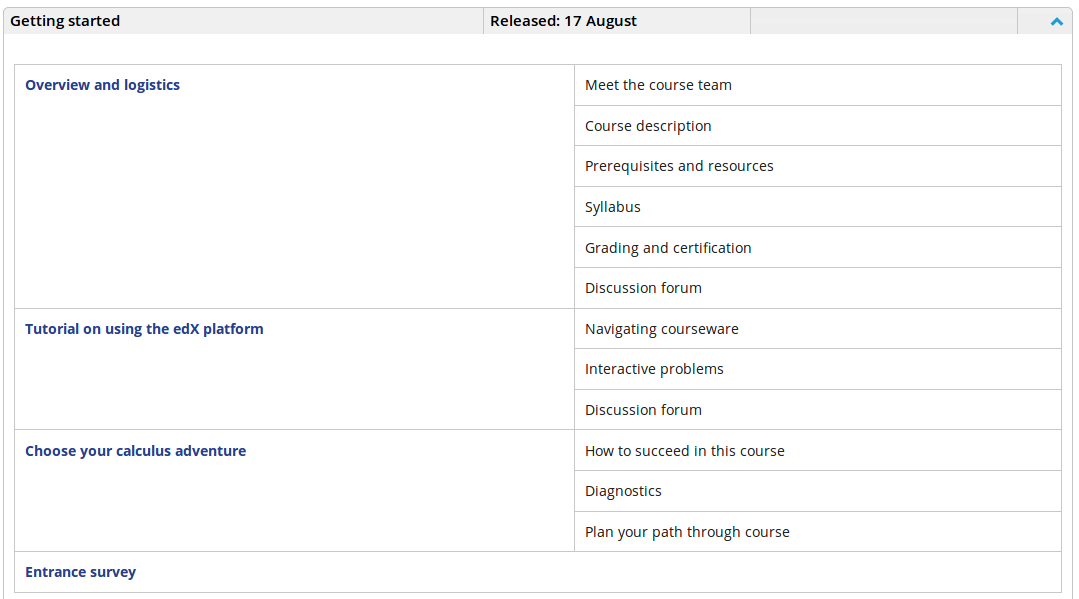
\includegraphics[scale=0.35]{imagens/syllabus1.png}}
  \end{center}
\end{figure}

\begin{figure}[H]
  \begin{center}
    %\caption{}
    \label{fig:syllabus2}
    \fbox{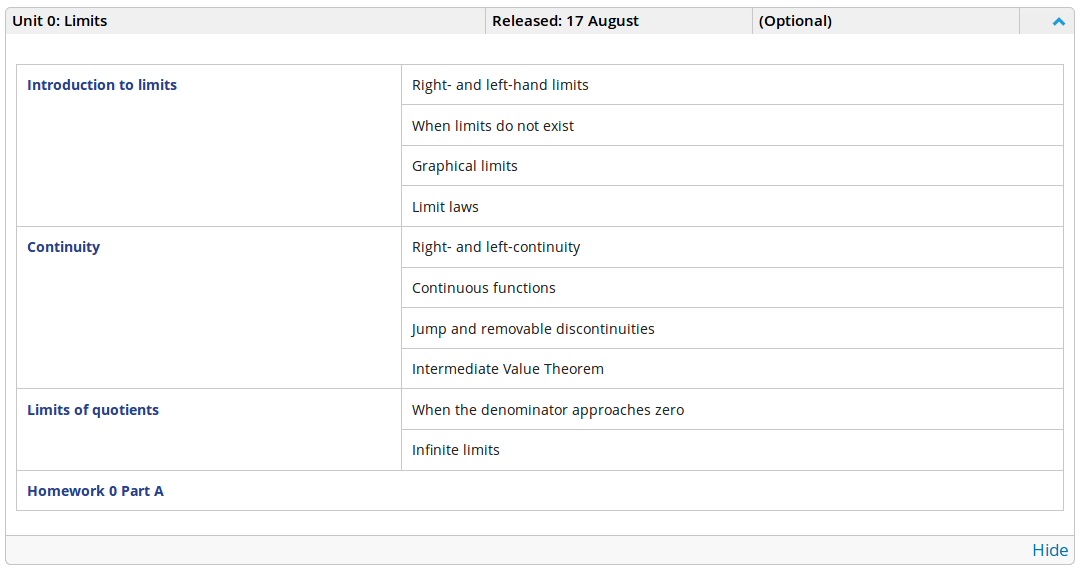
\includegraphics[scale=0.35]{imagens/syllabus2.png}}
  \end{center}
\end{figure}

\begin{figure}[H]
  \begin{center}
    %\caption{}
    \label{fig:syllabus3}
    \fbox{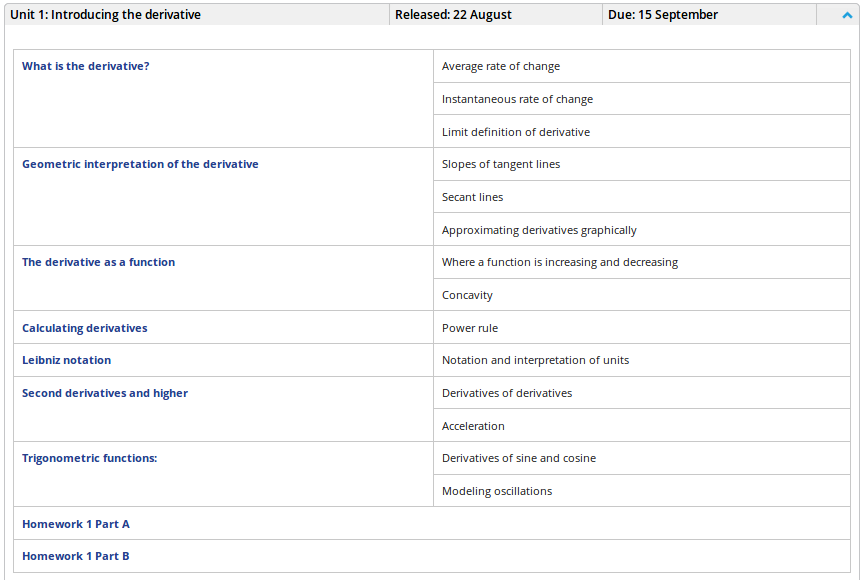
\includegraphics[scale=0.35]{imagens/syllabus3.png}}
  \end{center}
\end{figure}

\begin{figure}[H]
  \begin{center}
    %\caption{}
    \label{fig:syllabus4}
    \fbox{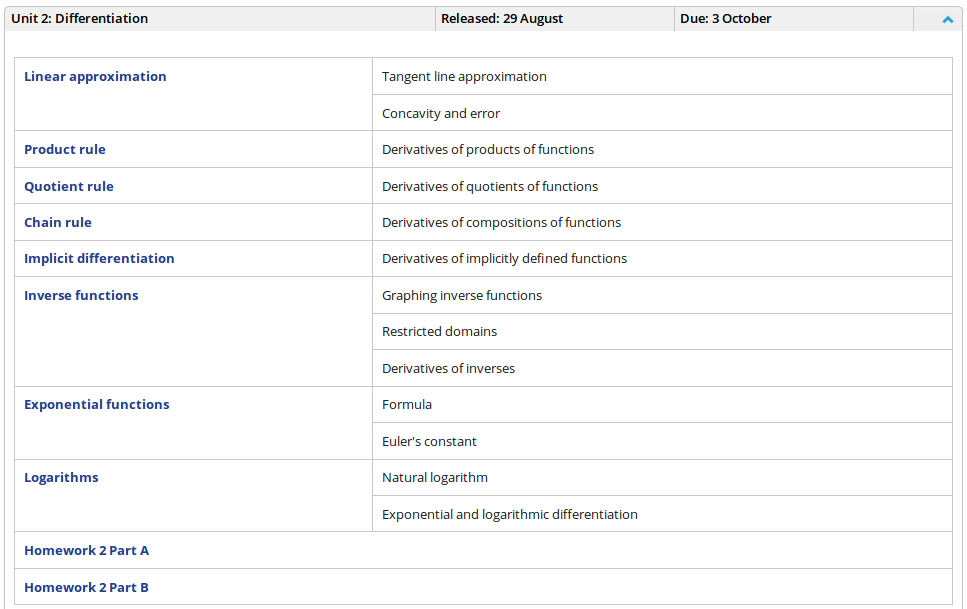
\includegraphics[scale=0.32]{imagens/syllabus4.png}}
  \end{center}
\end{figure}

\begin{figure}[H]
  \begin{center}
    %\caption{}
    \label{fig:syllabus5}
    \fbox{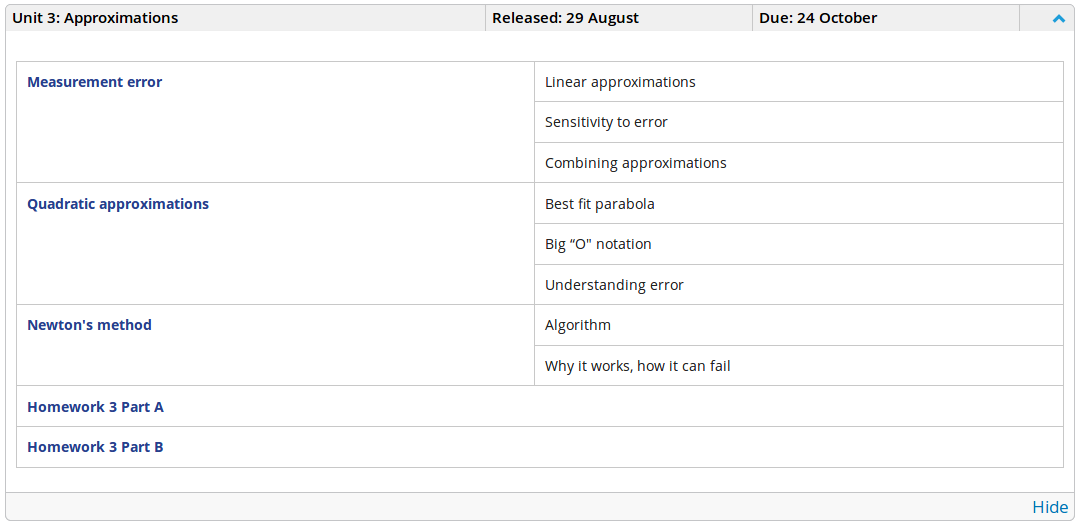
\includegraphics[scale=0.30]{imagens/syllabus5.png}}
  \end{center}
\end{figure}

\begin{figure}[H]
  \begin{center}
    %\caption{}
    \label{fig:syllabus6}
    \fbox{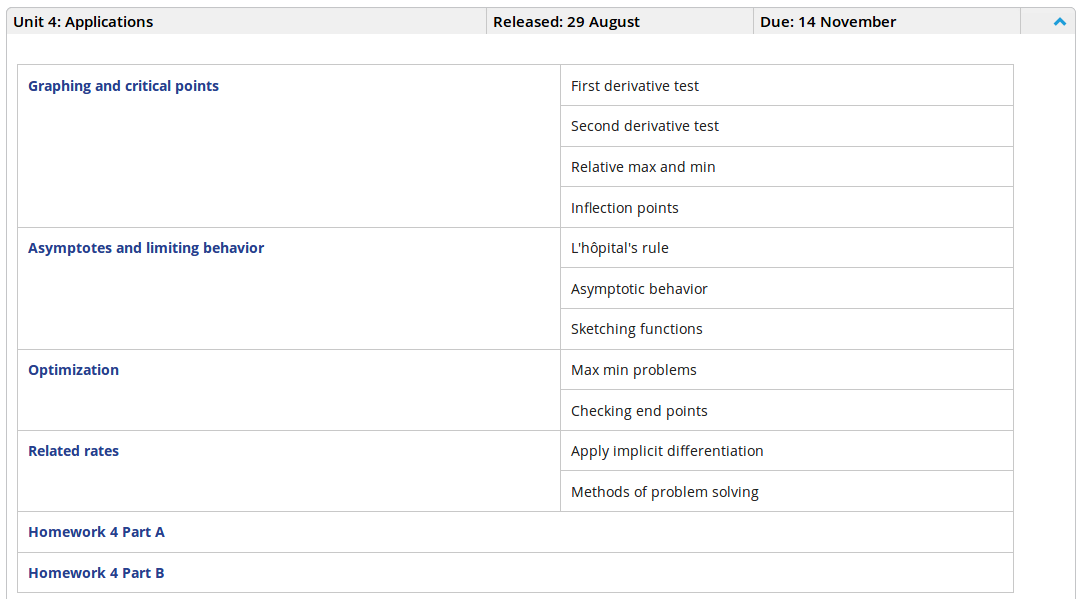
\includegraphics[scale=0.30]{imagens/syllabus6.png}}
  \end{center}
\end{figure}

\begin{figure}[H]
  \begin{center}
    %\caption{}
    \label{fig:syllabus7}
    \fbox{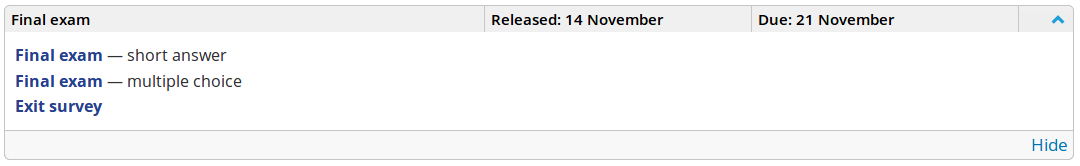
\includegraphics[scale=0.35]{imagens/syllabus7.png}}
  \end{center}
\end{figure}


%%%%%%%%%%%%%%%%%%%%%%%%%%%%%%%%%%%%%%%%%%%%%%%%%%%%%%%%%%%%%%%%%%%%%%%%%%%%%%%%%
%%%%%%%%%%%%%%%%%%%%%%%%%%%%%%%%%%%%%%%%%%%%%%%%%%%%%%%%%%%%%%%%%%%%%%%%%%%%%%%%%
\subsection{Entrance survey}
\label{gs-survey}

%%%%%%%%%%%%%%%%%%%%%%%%%%%%%%%%%%%%%%%%%%%%%%%%%%%%%%%%%%%%%%%%%%%%%%%%%%%%%%%%%
\subsubsection{Entrance survey}
\label{gs-survey-survey}

Welcome to this online course from MITx.

For us to offer the best course experience possible, we'd like to ask you to answer a few questions about yourself.

Whether you are just browsing or you are determined to complete the entire course, the more we know about you, the better we can serve all students in this course. As one of the first students in this new, free offering, your responses will be especially important to us. 

There are no right or wrong answers or responses, and your honest feedback is very important to us.  After reading the consent document below, you may click the right arrow below to proceed. 

\textbf{General Information About Survey Research in MITx. Please Read then Click Below to Continue.}

\textbf{Participation is voluntary}.
All survey responses are voluntary, students can skip any question at any time, and any responses have no effect on student assessments or participation. 

\textbf{What is the purpose of this research?}
We are interested in learning more about our participants’ backgrounds, interests, and motivations, and encouraging engagement with the course, so we can do the best possible job designing, evaluating and refining this course. With this research we will understand how to best encourage engagement with online education . 

\textbf{How long will I take part in this research?}
Your participation will be the duration of the course.

\textbf{What can I expect if I take part in this research?}
As a participant, you will be provided questions about yourself and other short prompts, which we will use to understand your participation in the course.  
 
\textbf{What are the risks and possible discomforts?}
If you choose to participate, we anticipate minimal risks and only the minor discomfort that might accompany online surveys. 

\textbf{Are there any benefits from being in this research study? }
We cannot promise any benefits to you or others from taking part in this research. However, possible benefits include your being more engaged with the course and better serving future students who participate in online courses. 

\textbf{If I take part in this research, how will my privacy be protected? What happens to the information you collect?}
Your instructor will not be able to identify your personal responses during the course and researchers will not attempt to identify individuals.  Your data will not be made identifiable to anyone other than researchers and course staff, and it will be aggregated for analysis and publication purposes. 

\textbf{If I have any questions, concerns or complaints about this research study, who can I talk to?}
The researcher for this study is Justin Reich who can be reached at 617-715-2962, 600 Technology Square, NE49-2028, Cambridge, MA, 02139, jreich@mit.edu for any of the following:
\begin{itemize}
\item If you have questions, concerns, or complaints,
\item If you would like to talk to the research team,
\item If you think the research has harmed you, or
\item If you wish to withdraw from the study.
\end{itemize}

This research has been reviewed by the Committee on the Use of Human Subjects in Research at Harvard University.  They can be reached at 617-496-2847, 1414 Massachusetts Avenue, Second Floor, Cambridge, MA 02138, or cuhs@fas.harvard.edu for any of the following:
\begin{itemize}
\item If your questions, concerns, or complaints are not being answered by the research team,
\item If you cannot reach the research team,
\item If you want to talk to someone besides the research team, or
\item If you have questions about your rights as a research participant.
\end{itemize}

Please print or save a copy of this form for your records.
\textbf{If you agree to participate, please click "Next" to enter the survey.}

\begin{figure}[H]
  \begin{center}
    %\caption{}
    \label{fig:survey01}
    \fbox{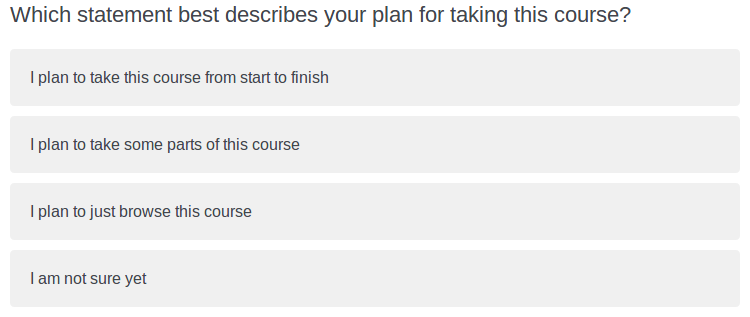
\includegraphics[scale=0.5]{imagens/survey01.png}}
  \end{center}
\end{figure}

\begin{figure}[H]
  \begin{center}
    %\caption{}
    \label{fig:survey02}
    \fbox{
\includegraphics[scale=0.5]{imagens/survey02.png}}
  \end{center}
\end{figure}

\begin{figure}[H]
  \begin{center}
    %\caption{}
    \label{fig:survey03}
    \fbox{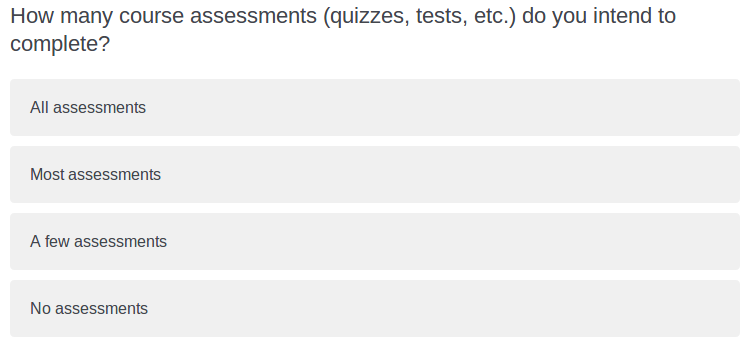
\includegraphics[scale=0.5]{imagens/survey03.png}}
  \end{center}
\end{figure}

\begin{figure}[H]
  \begin{center}
    %\caption{}
    \label{fig:survey04}
    \fbox{
\includegraphics[scale=0.5]{imagens/survey04.png}}
  \end{center}
\end{figure}

\begin{figure}[H]
  \begin{center}
    %\caption{}
    \label{fig:survey05}
    \fbox{
\includegraphics[scale=0.5]{imagens/survey05.png}}
  \end{center}
\end{figure}

\begin{figure}[H]
  \begin{center}
    %\caption{}
    \label{fig:survey06}
    \fbox{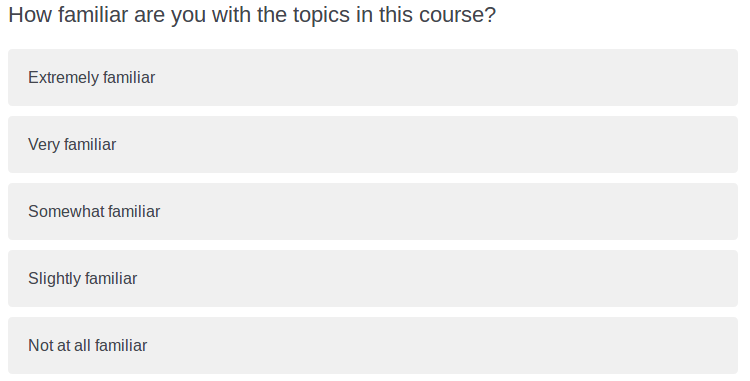
\includegraphics[scale=0.5]{imagens/survey06.png}}
  \end{center}
\end{figure}

\begin{figure}[H]
  \begin{center}
    %\caption{}
    \label{fig:survey07}
    \fbox{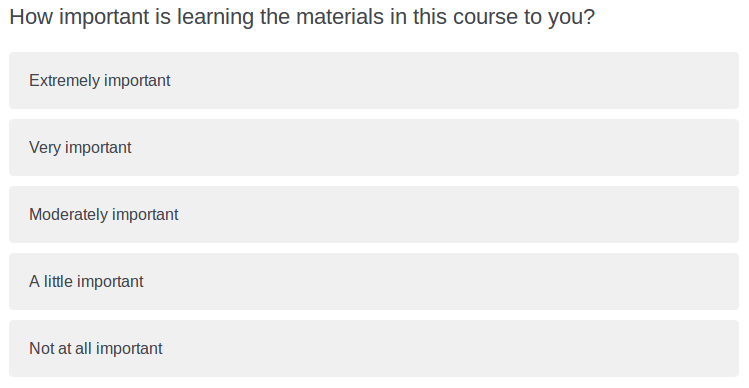
\includegraphics[scale=0.5]{imagens/survey07.png}}
  \end{center}
\end{figure}

\begin{figure}[H]
  \begin{center}
    %\caption{}
    \label{fig:survey08}
    \fbox{
\includegraphics[scale=0.5]{imagens/survey08.png}}
  \end{center}
\end{figure}

\begin{figure}[H]
  \begin{center}
    %\caption{}
    \label{fig:survey09}
    \fbox{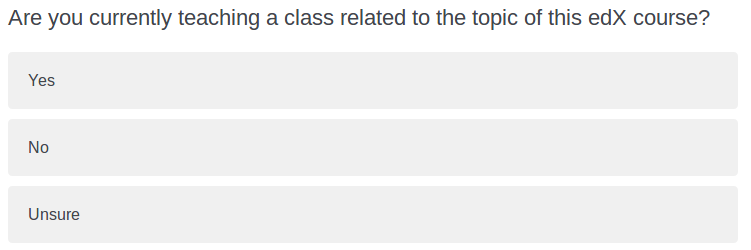
\includegraphics[scale=0.5]{imagens/survey09.png}}
  \end{center}
\end{figure}

\begin{figure}[H]
  \begin{center}
    %\caption{}
    \label{fig:survey10}
    \fbox{
\includegraphics[scale=0.5]{imagens/survey10.png}}
  \end{center}
\end{figure}

\begin{figure}[H]
  \begin{center}
    %\caption{}
    \label{fig:survey11}
    \fbox{
\includegraphics[scale=0.5]{imagens/survey11.png}}
  \end{center}
\end{figure}

\begin{figure}[H]
  \begin{center}
    %\caption{}
    \label{fig:survey12}
    \fbox{
\includegraphics[scale=0.5]{imagens/survey12.png}}
  \end{center}
\end{figure}

\begin{figure}[H]
  \begin{center}
    %\caption{}
    \label{fig:survey13}
    \fbox{
\includegraphics[scale=0.5]{imagens/survey13.png}}
  \end{center}
\end{figure}

\begin{figure}[H]
  \begin{center}
    %\caption{}
    \label{fig:survey14}
    \fbox{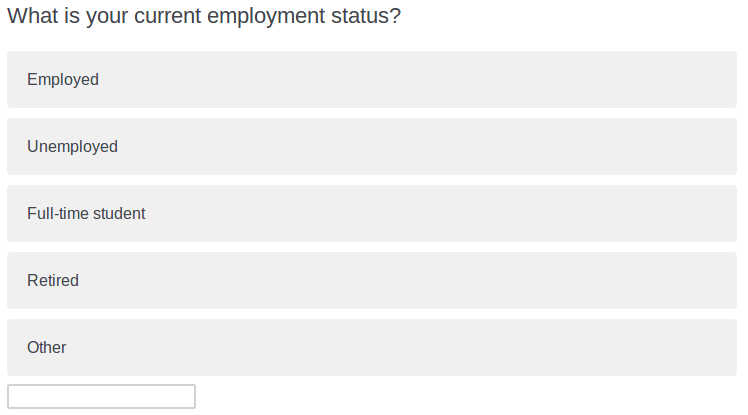
\includegraphics[scale=0.5]{imagens/survey14.png}}
  \end{center}
\end{figure}

\begin{figure}[H]
  \begin{center}
    %\caption{}
    \label{fig:survey15}
    \fbox{
\includegraphics[scale=0.5]{imagens/survey15.png}}
  \end{center}
\end{figure}

\begin{figure}[H]
  \begin{center}
    %\caption{}
    \label{fig:survey16}
    \fbox{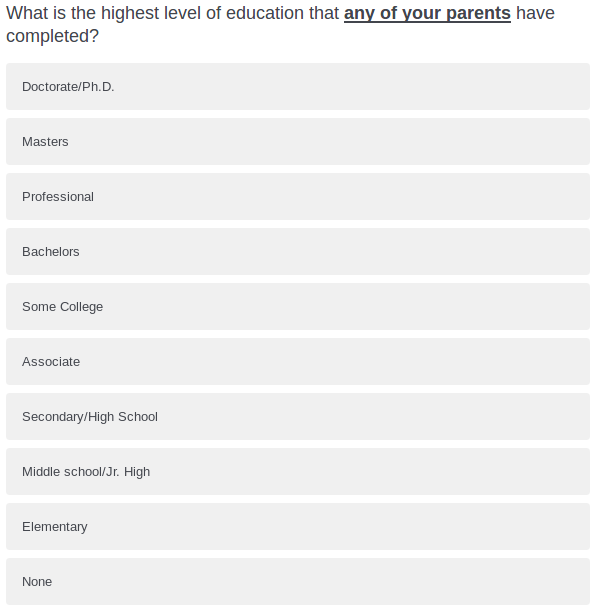
\includegraphics[scale=0.5]{imagens/survey16.png}}
  \end{center}
\end{figure}

\begin{figure}[H]
  \begin{center}
    %\caption{}
    \label{fig:survey17}
    \fbox{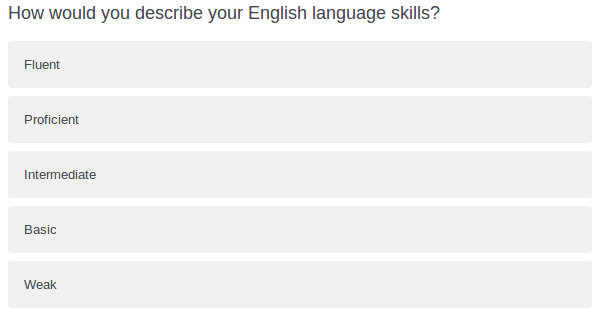
\includegraphics[scale=0.5]{imagens/survey17.png}}
  \end{center}
\end{figure}

\begin{figure}[H]
  \begin{center}
    %\caption{}
    \label{fig:survey18}
    \fbox{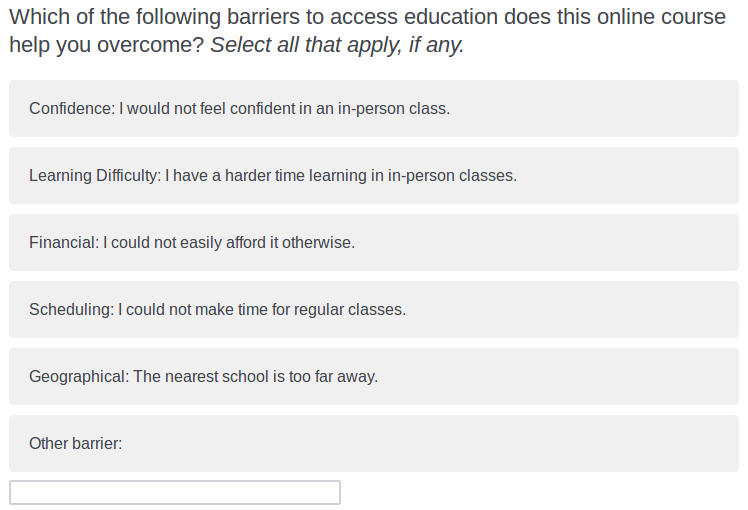
\includegraphics[scale=0.5]{imagens/survey18.png}}
  \end{center}
\end{figure}

\begin{figure}[H]
  \begin{center}
    %\caption{}
    \label{fig:survey19}
    \fbox{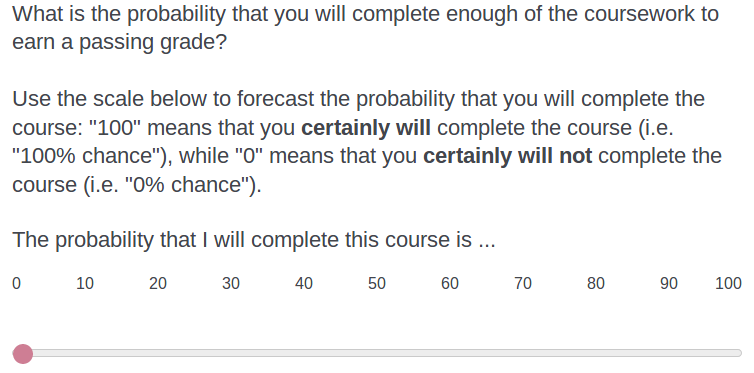
\includegraphics[scale=0.5]{imagens/survey19.png}}
  \end{center}
\end{figure}

\begin{figure}[H]
  \begin{center}
    %\caption{}
    \label{fig:survey20}
    \fbox{
\includegraphics[scale=0.5]{imagens/survey20.png}}
  \end{center}
\end{figure}

\begin{figure}[H]
  \begin{center}
    %\caption{}
    \label{fig:survey21}
    \fbox{
\includegraphics[scale=0.5]{imagens/survey21.png}}
  \end{center}
\end{figure}

\begin{figure}[H]
  \begin{center}
    %\caption{}
    \label{fig:survey22}
    \fbox{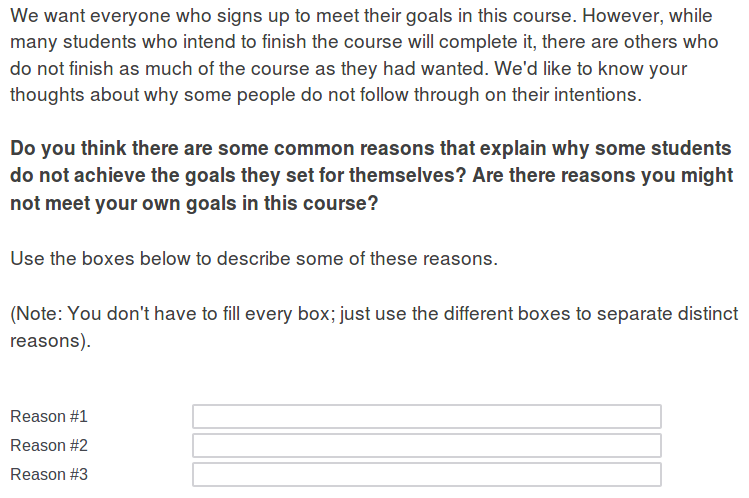
\includegraphics[scale=0.5]{imagens/survey22.png}}
  \end{center}
\end{figure}

\begin{figure}[H]
  \begin{center}
    %\caption{}
    \label{fig:survey23}
    \fbox{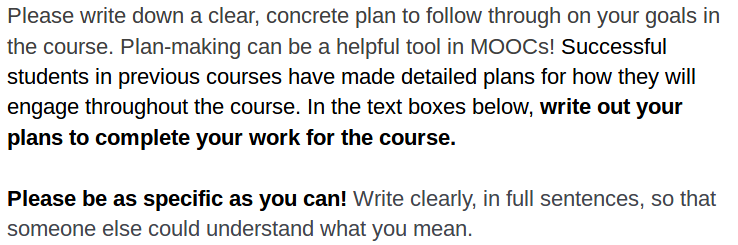
\includegraphics[scale=0.5]{imagens/survey23.png}}
  \end{center}
\end{figure}

\begin{figure}[H]
  \begin{center}
    %\caption{}
    \label{fig:survey24}
    \fbox{
\includegraphics[scale=0.5]{imagens/survey24.png}}
  \end{center}
\end{figure}

\begin{figure}[H]
  \begin{center}
    %\caption{}
    \label{fig:survey25}
    \fbox{
\includegraphics[scale=0.5]{imagens/survey25.png}}
  \end{center}
\end{figure}

\begin{figure}[H]
  \begin{center}
    %\caption{}
    \label{fig:survey26}
    \fbox{
\includegraphics[scale=0.5]{imagens/survey26.png}}
  \end{center}
\end{figure}




%%%%%%%%%%%%%%%%%%%%%%%%%%%%%%%%%%%%%%%%%%%%%%%%%%%%%%%%%%%%%%%%%%%%%%%%%%%%%%%%%
%%%%%%%%%%%%%%%%%%%%%%%%%%%%%%%%%%%%%%%%%%%%%%%%%%%%%%%%%%%%%%%%%%%%%%%%%%%%%%%%%
%%%%%%%%%%%%%%%%%%%%%%%%%%%%%%%%%%%%%%%%%%%%%%%%%%%%%%%%%%%%%%%%%%%%%%%%%%%%%%%%%
\newpage
\section{Unit 0: limits}
\label{u0}


%%%%%%%%%%%%%%%%%%%%%%%%%%%%%%%%%%%%%%%%%%%%%%%%%%%%%%%%%%%%%%%%%%%%%%%%%%%%%%%%%
%%%%%%%%%%%%%%%%%%%%%%%%%%%%%%%%%%%%%%%%%%%%%%%%%%%%%%%%%%%%%%%%%%%%%%%%%%%%%%%%%
\subsection{Introduction to limits}
\label{u0-intro}

%%%%%%%%%%%%%%%%%%%%%%%%%%%%%%%%%%%%%%%%%%%%%%%%%%%%%%%%%%%%%%%%%%%%%%%%%%%%%%%%%
\subsubsection{Motivation}
\label{u0-intro-motiv}

Video: \href{https://www.youtube.com/watch?v=nh5O6-2Evk8}{Introduction to Limits}

Calculus has two main concepts --- the derivative
and the integral.
But in order to understand either of them,
you first have to understand limits.

So let's talk limits.
We'll start with a curve.
Fix a point A on the curve.
Choose a second point, B, which we're going to move.
And draw a line through A and B. Let's look
at what happens when B moves closer and closer to the point
A.

This is an example of a limit.
In the limit, the line becomes tangent to the curve
at the point A. The slope of this line
is the derivative at the point A. Now let's see how limits
are related to integrals.

Integrals are used to measure areas of curvy regions
like this.
Measuring areas of curvy regions seems hard,
but measuring areas of rectangles
is easy, so we'll try to fill our region with rectangles.

Each rectangle has a certain width.
As we make the width smaller, the total area
of the rectangles gets closer and closer
to the area of the curvy region.

The integral is the limit of the total area of the rectangles
as the width tends to zero.

So that's why we start with limits.
They're the foundation for everything else in calculus.
At the beginning, limits may seem abstract,
but very quickly you'll get used to them.

%%%%%%%%%%%%%%%%%%%%%%%%%%%%%%%%%%%%%%%%%%%%%%%%%%%%%%%%%%%%%%%%%%%%%%%%%%%%%%%%%
\subsubsection{Introduction to limits}
\label{u0-intro-intro}

\paragraph{Objectives} At the end of this sequence, and after some practice, you should be able to:
\begin{itemize}[noitemsep]
\item Use a calculator to determine right and left hand limits.
\item Identify right and left hand limits based on graphs.
\item Determine if a limit exists based on values of right and left hand limits.
\item Understand that the limit does not depend on the value of a function at the point of interest.
\end{itemize}

Contents: 14 pages, 6 videos (24 minutes 1x speed), 17 questions.

%%%%%%%%%%%%%%%%%%%%%%%%%%%%%%%%%%%%%%%%%%%%%%%%%%%%%%%%%%%%%%%%%%%%%%%%%%%%%%%%%
\subsubsection{Moving closer and closer}
\label{u0-intro-moving}

Video: \href{https://www.youtube.com/watch?v=bANtYKLugsU}{Moving closer and closer}

Welcome.

Calculus is all about functions. You probably know that a function f takes an input x
and gives an output f of x. But in calculus, we're not concerned with just one input
and finding the output for that one input. We want to consider a whole range of inputs.
So we would want to know what happens when the input "moves" or "varies."
For instance, we could ask what happens as the input moves really close.
Closer and closer to some point. Let's say 1.

And to be even more specific, let's say that x is moving towards 1 from the left.
So if this is a number line, and we've got the point 1 right there, then x
could start here, and just move closer and closer and closer towards 1, from the left.
We'll use this arrow notation to denote that x is getting really, really close to 1.
But a warning, this does not mean that x will ever actually equal 1.
We're only concerned with values of x that are near one.

OK. Now that that's said, as x moves,
we know that the output f of x is also going to move.
And so the question that we can ask
is as x moves closer and closer to 1 from the left,
does f of x move closer and closer
to some value of its own?

Let's be concrete here.
And pick a particular function f.
I'm going to choose f of x to be the square root of 3 minus 5 x
plus x squared, plus x cubed, all over x minus 1.
Kind of a complicated function, but you'll
have to trust me that this is a good example.
And what we can do in order to see what's
happening to f as x approaches 1 from the left
is just select certain values of x
that are getting closer and closer to 1 from the left.
So over here on the number line, we
could start with x equals zero.
And then they get closer, we could try x equals 0.5.
Or even closer, maybe 0.9.
Even 0.99.
These sorts of values.
And we want to know, what's happening to the output?
So we can just plug these values into the function,
and see whether the output gets closer and closer to anything.

Now there are technically infinitely many values
of x that we could have chosen here.
But let's just start with these four.
Remember though that one value of x
that we will definitely not consider
is x equal to 1 itself.
In fact, this function isn't even defined at x equals 1.
We'd have a zero denominator.
It is, however, defined when x is approaching one,
and those are the values we're considering.

OK.
Well let's make a table with our chosen
inputs and the associated outputs,
and let's just calculate those outputs.
So when we plug in zero we'll get a square root of 3
on top divided by minus 1.
So minus square root of 3, which is roughly minus 1.73.
Next up is x equals 0.5.
I'm going to have to bust out the calculator here.
So we've got 3 minus 5 times 0.5 plus 0.5 squared
plus 0.5 cubed, and then we need the square root,
and then we need to divide by 0.5 minus 1.
So 0.5 negative.
So we get minus 1.87, roughly.
So back to our table.
We've got f of x moving from minus 1.73 to minus 1.87.
Well that's not really enough data
to tell if f is getting closer and closer to anything
in particular.
So let's take our next two values of x and plug those in.
I'm going to fast forward through the calculations.
You ready?
x equals 0.9.
All right?
That's approximately minus 1.97, and finally 0.99,
and we've got minus 1.997.
So as we go down this table, f of x
is getting really, really close to what looks like minus 2.
So we can say that as x approaches 1 from the left,
f of x approaches minus 2.
Now f of x might never actually equal to minus 2,
just as x never actually equals one,
but it gets really, really close.
And if it gets arbitrarily close,
meaning as close as we could possibly want,
then that's really all we'll care about.
What I would like you to do now is
to do this same exercise, except this time have x approach 1
from the right.
You might be surprised at what you find.
We'll talk afterwards.

Determine what happens to $\displaystyle f(x) = \frac{\sqrt{3-5x+x^2+x^3}}{x-1}$ as $x$ approaches $1$ from the right.
Take values of $x$ that are greater than 1, but getting closer and closer to 1. For instance, you could try
$x=1.1, 1.01, 1.001, 1.0001$, etc. What happens to $f(x)$ as $x$ approaches 1 from the right?

\begin{itemize}[noitemsep]
\item[$\square$] $f(x)$ gets closer and closer to a particular number
\item[$\square$] $f(x)$ gets bigger and bigger in the positive direction without bound
\item[$\square$] $f(x)$ gets bigger and bigger in the negative direction without bound
\item[$\square$] None of the above
\end{itemize}

What value does $f(x)$ get closer to? Enter the number below;
if there is no such value, enter capital (for "does not exist")

%%%%%%%%%%%%%%%%%%%%%%%%%%%%%%%%%%%%%%%%%%%%%%%%%%%%%%%%%%%%%%%%%%%%%%%%%%%%%%%%%
\subsubsection{One-sided limits}
\label{u0-intro-one-sided}

Video: \href{https://www.youtube.com/watch?v=fAAzAVHVKQk}{One-sided limits}

%%%%%%%%%%%%%%%%%%%%%%%%%%%%%%%%%%%%%%%%%%%%%%%%%%%%%%%%%%%%%%%%%%%%%%%%%%%%%%%%%
\subsubsection{Definitions of right-hand and left-hand limits}
\label{u0-intro-right-left}

%%%%%%%%%%%%%%%%%%%%%%%%%%%%%%%%%%%%%%%%%%%%%%%%%%%%%%%%%%%%%%%%%%%%%%%%%%%%%%%%%
\subsubsection{A few more limits}
\label{u0-intro-more}

xx

%%%%%%%%%%%%%%%%%%%%%%%%%%%%%%%%%%%%%%%%%%%%%%%%%%%%%%%%%%%%%%%%%%%%%%%%%%%%%%%%%
\subsubsection{Possible limits behaviors}
\label{u0-intro-behaviors}

xx

%%%%%%%%%%%%%%%%%%%%%%%%%%%%%%%%%%%%%%%%%%%%%%%%%%%%%%%%%%%%%%%%%%%%%%%%%%%%%%%%%
\subsubsection{Quick limit questions}
\label{u0-intro-questions}

xx

%%%%%%%%%%%%%%%%%%%%%%%%%%%%%%%%%%%%%%%%%%%%%%%%%%%%%%%%%%%%%%%%%%%%%%%%%%%%%%%%%
\subsubsection{The overall limit}
\label{u0-intro-overall}

xx

%%%%%%%%%%%%%%%%%%%%%%%%%%%%%%%%%%%%%%%%%%%%%%%%%%%%%%%%%%%%%%%%%%%%%%%%%%%%%%%%%
\subsubsection{Limit definition}
\label{u0-intro-definition}

xx

%%%%%%%%%%%%%%%%%%%%%%%%%%%%%%%%%%%%%%%%%%%%%%%%%%%%%%%%%%%%%%%%%%%%%%%%%%%%%%%%%
\subsubsection{Limits from graphs}
\label{u0-intro-graphs}

xx

%%%%%%%%%%%%%%%%%%%%%%%%%%%%%%%%%%%%%%%%%%%%%%%%%%%%%%%%%%%%%%%%%%%%%%%%%%%%%%%%%
\subsubsection{Review problems}
\label{u0-intro-review}

xx

%%%%%%%%%%%%%%%%%%%%%%%%%%%%%%%%%%%%%%%%%%%%%%%%%%%%%%%%%%%%%%%%%%%%%%%%%%%%%%%%%
\subsubsection{Limit laws}
\label{u0-intro-laws}

xx

%%%%%%%%%%%%%%%%%%%%%%%%%%%%%%%%%%%%%%%%%%%%%%%%%%%%%%%%%%%%%%%%%%%%%%%%%%%%%%%%%
\subsubsection{Limit laws (2)}
\label{u0-intro-laws2}

xx

%%%%%%%%%%%%%%%%%%%%%%%%%%%%%%%%%%%%%%%%%%%%%%%%%%%%%%%%%%%%%%%%%%%%%%%%%%%%%%%%%
\subsubsection{Summary}
\label{u0-intro-summary}

xx


%%%%%%%%%%%%%%%%%%%%%%%%%%%%%%%%%%%%%%%%%%%%%%%%%%%%%%%%%%%%%%%%%%%%%%%%%%%%%%%%%
%%%%%%%%%%%%%%%%%%%%%%%%%%%%%%%%%%%%%%%%%%%%%%%%%%%%%%%%%%%%%%%%%%%%%%%%%%%%%%%%%
\subsection{Continuity}
\label{u0-cont}

%%%%%%%%%%%%%%%%%%%%%%%%%%%%%%%%%%%%%%%%%%%%%%%%%%%%%%%%%%%%%%%%%%%%%%%%%%%%%%%%%
\subsubsection{Motivation}
\label{u0-cont-motivation}

xx

%%%%%%%%%%%%%%%%%%%%%%%%%%%%%%%%%%%%%%%%%%%%%%%%%%%%%%%%%%%%%%%%%%%%%%%%%%%%%%%%%
\subsubsection{How do we compute limits?}
\label{u0-cont-how-compute}

xx

%%%%%%%%%%%%%%%%%%%%%%%%%%%%%%%%%%%%%%%%%%%%%%%%%%%%%%%%%%%%%%%%%%%%%%%%%%%%%%%%%
\subsubsection{Continuity}
\label{u0-cont-continuity}

xx

%%%%%%%%%%%%%%%%%%%%%%%%%%%%%%%%%%%%%%%%%%%%%%%%%%%%%%%%%%%%%%%%%%%%%%%%%%%%%%%%%
\subsubsection{Continuity questions}
\label{u0-cont-continuity-questions}

xx

%%%%%%%%%%%%%%%%%%%%%%%%%%%%%%%%%%%%%%%%%%%%%%%%%%%%%%%%%%%%%%%%%%%%%%%%%%%%%%%%%
\subsubsection{More continuity questions}
\label{u0-cont-more-continuity-questions}

xx

%%%%%%%%%%%%%%%%%%%%%%%%%%%%%%%%%%%%%%%%%%%%%%%%%%%%%%%%%%%%%%%%%%%%%%%%%%%%%%%%%
\subsubsection{Overall continuity}
\label{u0-cont-overall}

xx

%%%%%%%%%%%%%%%%%%%%%%%%%%%%%%%%%%%%%%%%%%%%%%%%%%%%%%%%%%%%%%%%%%%%%%%%%%%%%%%%%
\subsubsection{Continuity continued}
\label{u0-cont-continuity-continued}

xx

%%%%%%%%%%%%%%%%%%%%%%%%%%%%%%%%%%%%%%%%%%%%%%%%%%%%%%%%%%%%%%%%%%%%%%%%%%%%%%%%%
\subsubsection{Limit laws and continuity}
\label{u0-cont-laws}

xx

%%%%%%%%%%%%%%%%%%%%%%%%%%%%%%%%%%%%%%%%%%%%%%%%%%%%%%%%%%%%%%%%%%%%%%%%%%%%%%%%%
\subsubsection{Review of continuity}
\label{u0-cont-review}

xx

%%%%%%%%%%%%%%%%%%%%%%%%%%%%%%%%%%%%%%%%%%%%%%%%%%%%%%%%%%%%%%%%%%%%%%%%%%%%%%%%%
\subsubsection{Catalog of continuous functions}
\label{u0-cont-catalog}

xx

%%%%%%%%%%%%%%%%%%%%%%%%%%%%%%%%%%%%%%%%%%%%%%%%%%%%%%%%%%%%%%%%%%%%%%%%%%%%%%%%%
\subsubsection{IVT intro}
\label{u0-cont-ivt}

xx

%%%%%%%%%%%%%%%%%%%%%%%%%%%%%%%%%%%%%%%%%%%%%%%%%%%%%%%%%%%%%%%%%%%%%%%%%%%%%%%%%
\subsubsection{Intermediate Value Theorem}
\label{u0-cont-intermediate-value-theorem}

xx

%%%%%%%%%%%%%%%%%%%%%%%%%%%%%%%%%%%%%%%%%%%%%%%%%%%%%%%%%%%%%%%%%%%%%%%%%%%%%%%%%
\subsubsection{Basics}
\label{u0-cont-basics}

xx

%%%%%%%%%%%%%%%%%%%%%%%%%%%%%%%%%%%%%%%%%%%%%%%%%%%%%%%%%%%%%%%%%%%%%%%%%%%%%%%%%
\subsubsection{Roots}
\label{u0-cont-roots}

xx

%%%%%%%%%%%%%%%%%%%%%%%%%%%%%%%%%%%%%%%%%%%%%%%%%%%%%%%%%%%%%%%%%%%%%%%%%%%%%%%%%
\subsubsection{Summary}
\label{u0-cont-summary}

xx


%%%%%%%%%%%%%%%%%%%%%%%%%%%%%%%%%%%%%%%%%%%%%%%%%%%%%%%%%%%%%%%%%%%%%%%%%%%%%%%%%
%%%%%%%%%%%%%%%%%%%%%%%%%%%%%%%%%%%%%%%%%%%%%%%%%%%%%%%%%%%%%%%%%%%%%%%%%%%%%%%%%
\subsection{Limits of quotients}
\label{u0-lim-quo}

%%%%%%%%%%%%%%%%%%%%%%%%%%%%%%%%%%%%%%%%%%%%%%%%%%%%%%%%%%%%%%%%%%%%%%%%%%%%%%%%%
\subsubsection{Limits of quotients}
\label{u0-lim-quo-lim}

xx

%%%%%%%%%%%%%%%%%%%%%%%%%%%%%%%%%%%%%%%%%%%%%%%%%%%%%%%%%%%%%%%%%%%%%%%%%%%%%%%%%
\subsubsection{How do we compute limits of quotients?}
\label{u0-lim-quo-how-compute}

xx

%%%%%%%%%%%%%%%%%%%%%%%%%%%%%%%%%%%%%%%%%%%%%%%%%%%%%%%%%%%%%%%%%%%%%%%%%%%%%%%%%
\subsubsection{Limits and division}
\label{u0-lim-quo-lim-div}

xx

%%%%%%%%%%%%%%%%%%%%%%%%%%%%%%%%%%%%%%%%%%%%%%%%%%%%%%%%%%%%%%%%%%%%%%%%%%%%%%%%%
\subsubsection{Quotients of small numbers}
\label{u0-lim-quo-small}

xx

%%%%%%%%%%%%%%%%%%%%%%%%%%%%%%%%%%%%%%%%%%%%%%%%%%%%%%%%%%%%%%%%%%%%%%%%%%%%%%%%%
\subsubsection{Small divided by small}
\label{u0-lim-quo-small-div-small}

xx

%%%%%%%%%%%%%%%%%%%%%%%%%%%%%%%%%%%%%%%%%%%%%%%%%%%%%%%%%%%%%%%%%%%%%%%%%%%%%%%%%
\subsubsection{Limit law for division}
\label{u0-lim-quo-limit-law-div}

xx

%%%%%%%%%%%%%%%%%%%%%%%%%%%%%%%%%%%%%%%%%%%%%%%%%%%%%%%%%%%%%%%%%%%%%%%%%%%%%%%%%
\subsubsection{Limit laws}
\label{u0-lim-quo-limit-laws}

xx

%%%%%%%%%%%%%%%%%%%%%%%%%%%%%%%%%%%%%%%%%%%%%%%%%%%%%%%%%%%%%%%%%%%%%%%%%%%%%%%%%
\subsubsection{Using the division limit law}
\label{u0-lim-quo-using-law}

xx

%%%%%%%%%%%%%%%%%%%%%%%%%%%%%%%%%%%%%%%%%%%%%%%%%%%%%%%%%%%%%%%%%%%%%%%%%%%%%%%%%
\subsubsection{Division limit questions}
\label{u0-lim-quo-questions}

xx

%%%%%%%%%%%%%%%%%%%%%%%%%%%%%%%%%%%%%%%%%%%%%%%%%%%%%%%%%%%%%%%%%%%%%%%%%%%%%%%%%
\subsubsection{Review problems}
\label{u0-lim-quo-review-prob}

xx

%%%%%%%%%%%%%%%%%%%%%%%%%%%%%%%%%%%%%%%%%%%%%%%%%%%%%%%%%%%%%%%%%%%%%%%%%%%%%%%%%
\subsubsection{Limits that don't exist}
\label{u0-lim-quo-dont-exist}

xx

%%%%%%%%%%%%%%%%%%%%%%%%%%%%%%%%%%%%%%%%%%%%%%%%%%%%%%%%%%%%%%%%%%%%%%%%%%%%%%%%%
\subsubsection{Another function}
\label{u0-lim-quo-another}

xx

%%%%%%%%%%%%%%%%%%%%%%%%%%%%%%%%%%%%%%%%%%%%%%%%%%%%%%%%%%%%%%%%%%%%%%%%%%%%%%%%%
\subsubsection{Infinite limits 2}
\label{u0-lim-quo-inf2}

xx

%%%%%%%%%%%%%%%%%%%%%%%%%%%%%%%%%%%%%%%%%%%%%%%%%%%%%%%%%%%%%%%%%%%%%%%%%%%%%%%%%
\subsubsection{What is the limit?}
\label{u0-lim-quo-what}

xx

%%%%%%%%%%%%%%%%%%%%%%%%%%%%%%%%%%%%%%%%%%%%%%%%%%%%%%%%%%%%%%%%%%%%%%%%%%%%%%%%%
\subsubsection{Division involving infinite limits}
\label{u0-lim-quo-div-inf}

xx

%%%%%%%%%%%%%%%%%%%%%%%%%%%%%%%%%%%%%%%%%%%%%%%%%%%%%%%%%%%%%%%%%%%%%%%%%%%%%%%%%
\subsubsection{Summary}
\label{u0-lim-quo-summary}

xx


%%%%%%%%%%%%%%%%%%%%%%%%%%%%%%%%%%%%%%%%%%%%%%%%%%%%%%%%%%%%%%%%%%%%%%%%%%%%%%%%%
%%%%%%%%%%%%%%%%%%%%%%%%%%%%%%%%%%%%%%%%%%%%%%%%%%%%%%%%%%%%%%%%%%%%%%%%%%%%%%%%%
\subsection{Homework Unit 0: Part A}
\label{u0-hw-pA}

%%%%%%%%%%%%%%%%%%%%%%%%%%%%%%%%%%%%%%%%%%%%%%%%%%%%%%%%%%%%%%%%%%%%%%%%%%%%%%%%%
\subsubsection{Part A Problems}
\label{u0-hw-pA-problems}

xx

%%%%%%%%%%%%%%%%%%%%%%%%%%%%%%%%%%%%%%%%%%%%%%%%%%%%%%%%%%%%%%%%%%%%%%%%%%%%%%%%%
\subsubsection{Part A Homework}
\label{u0-hw-pA-homework}

xx




%%%%%%%%%%%%%%%%%%%%%%%%%%%%%%%%%%%%%%%%%%%%%%%%%%%%%%%%%%%%%%%%%%%%%%%%%%%%%%%%%
%%%%%%%%%%%%%%%%%%%%%%%%%%%%%%%%%%%%%%%%%%%%%%%%%%%%%%%%%%%%%%%%%%%%%%%%%%%%%%%%%
%%%%%%%%%%%%%%%%%%%%%%%%%%%%%%%%%%%%%%%%%%%%%%%%%%%%%%%%%%%%%%%%%%%%%%%%%%%%%%%%%
\newpage
\section{Unit 1: The Derivative (2018/08/29)}
\label{u1}


%%%%%%%%%%%%%%%%%%%%%%%%%%%%%%%%%%%%%%%%%%%%%%%%%%%%%%%%%%%%%%%%%%%%%%%%%%%%%%%%%
%%%%%%%%%%%%%%%%%%%%%%%%%%%%%%%%%%%%%%%%%%%%%%%%%%%%%%%%%%%%%%%%%%%%%%%%%%%%%%%%%
\subsection{What is the derivative?}
\label{u1-what}

%%%%%%%%%%%%%%%%%%%%%%%%%%%%%%%%%%%%%%%%%%%%%%%%%%%%%%%%%%%%%%%%%%%%%%%%%%%%%%%%%
\subsubsection{What is the derivative?}
\label{u1-what-what}

Video: \href{https://www.youtube.com/watch?v=MCxsXQKNd-U}{What is the derivative?}

I just got a speeding ticket in the mail.
There were no police present on the turnpike, so my question for you is, how did
they know I was speeding?

What I can tell you is that I went
through the toll booth at the 50 mile marker at eight AM.
I went through a second toll booth at the 220 mile marker
at ten AM.
And by the way, I was certainly going slower than the speed
limit through the toll booths.

In this lesson, you'll figure out
why I got this speeding ticket.
We'll learn about average velocity,
instantaneous velocity, and explore
the relationship between them.

This relationship is crucial to the definition
of the derivative; and the derivative
is the subject of this entire course.

Note: In the United States, you cannot actually get a speeding ticket this way.
A law was passed that prevents law enforcement from using toll booth data to give
speeding tickets retroactively. Otherwise, no one would purchase automated
toll booth passes!

%%%%%%%%%%%%%%%%%%%%%%%%%%%%%%%%%%%%%%%%%%%%%%%%%%%%%%%%%%%%%%%%%%%%%%%%%%%%%%%%%
\subsubsection{Objectives}
\label{u1-what-obj}

\begin{itemize}[noitemsep]
\item Describe what is meant by an \emph{average rate of change}, and compute
  them with appropriate \emph{units}.
\item Describe the difference and relationship between the average rate of change
  and an \emph{instantaneous rate of change}.
\item Use a \emph{limit} to find the instantaneous rate of change, also known
  as the \emph{derivative} at a point.
\item Interpret the \emph{sign of a derivative} --- positive, negative, or zero
  --- as having real-world meaning.
\end{itemize}

Contents: 13 pages; 6 videos (23 minutes 1x speed); 17 questions.

%%%%%%%%%%%%%%%%%%%%%%%%%%%%%%%%%%%%%%%%%%%%%%%%%%%%%%%%%%%%%%%%%%%%%%%%%%%%%%%%%
\subsubsection{Rates of change}
\label{u1-what-rates-of-change}

Derivatives are all about rates of change. What do we mean by a rate of change?
Let's take an example.

Using the fact that you went through the toll booth at the 50 mile marker on the
Turnpike at 8am, and you went through a second toll booth at the 220 mile marker
at 10am.

\begin{exercise}
  \textbf{Average rate:} On average, how fast were you traveling between 8 AM and 10 AM?
\end{exercise}

\begin{exercise}
  \textbf{Check units:} OK, you entered a number there, and hopefully you got
  the right answer. But this is supposed to be measuring something real --- a velocity,
  not just a number. In what units did we just measure our speed?
\begin{itemize}[noitemsep]
\item[$\square$] kilometers
\item[$\square$] miles
\item[$\square$] hours
\item[$\square$] kilometers per hour
\item[$\square$] miles por hour
\item[$\square$] hours per kilometer
\item[$\square$] hours per mile
\item[$\square$] something else
\end{itemize}
\end{exercise}

%%%%%%%%%%%%%%%%%%%%%%%%%%%%%%%%%%%%%%%%%%%%%%%%%%%%%%%%%%%%%%%%%%%%%%%%%%%%%%%%%
\subsubsection{Average vs. Instantaneous}
\label{u1-what-avg-inst}

\begin{exercise}
  \textbf{Average:} We calculated a velocity of 85 miles per hour, so we were
  definitely speeding. Does that mean that at the exact instant of 8 AM, the speed
  of the car was exactly 85 mph?
\begin{itemize}[noitemsep]
\item[$\square$] yes
\item[$\square$] no
\end{itemize}
\end{exercise}

\begin{exercise}
  \textbf{Instantaneous approximation:} Which of the following would give us a
  better idea of the velocity at 8am?
\begin{itemize}[noitemsep]
\item[$\square$] Do the same calculation, but between 8am and 12pm instead of
  between 8am and 10am.
\item[$\square$] Do the same calculation, but between 8am and 8:01am instead
  of between 8am and 10am
\end{itemize}
\end{exercise}

Video: \href{https://www.youtube.com/watch?v=BBvacxW-h7M}{Average Velocity}

OK, we've calculated the average velocity
of our car between 8:00 and 10:00.
But then we decided that that might not
be such a good approximation if we wanted
the velocity at 8:00 exactly.
So we've decided that instead, we
should do the same calculation just this time,
between 8:00 and 8:01.

All right, we're going to have a lot of numbers floating around
here.
So let's get some notation to organize all this.
We know that position is a function of time.
So if we have $t$ as representing time,
then we can say that $f(t)$ is position.

So our initial data was that our position at 8:00 was 50 miles.
So $f(8) = 50$. And our position at 10:00 was 220 miles.

Now previously, you had used this data
to calculate that the average velocity between 8:00 and 10:00
was 85 miles per hour.
And that 85 came from 220 minus 50.
So we traveled 170 miles.
And then you divide by 10 minus 8.
That was the time, two hours, that the journey took.

So in our new notation, this is $f(10) - f(8)$
on top divided by $10 - 8$.
So our numerator here is the change in position.
And our denominator is the change in time.
And when you divide those two, we
get our average velocity of 85 miles per hour.

Now, calculus is all about variables changing, just
all over the place.
And so we have a special notation
that we use to denote the change in a variable.
So here, this numerator where we're
saying the change in position, or the change in f,
we often denote that by $\Delta f$.
So Delta ($\Delta$), this Greek letter here, this triangle,
stands for difference.

And so we have the difference in f.
This is not $\Delta \times f$.
Delta isn't a thing in and of itself.
It's just one quantity, $\Delta f$.

And similarly, on the denominator,
we're going to have a quantity, $\Delta t$, the change in time.

So this $\frac{\Delta f}{\Delta t}$
is giving us our average velocity over the period
of time from 8:00 to 10:00.

Now, we wanted to talk about 8:01.
So in order to do that, I need to tell you the position
of the car at 8:01.
And in our notation, that's going to be $f(8 + \frac{1}{60})$.
So that's 8 and 1/60 hours.
And let's say that the car was at mile marker 51
at that moment.

So given that information, what would you say
is the average velocity of the car between 8:00 and 8:01?
Why don't you think about that, and then
we'll come back and discuss some more.

\begin{exercise}
  \textbf{Average velocity 2:} Given that at 8:00 our position was 50 miles,
  and at 8:01 our position was 51 miles, what was our average velocity over
  the one minute from 8:00 to 8:01? Express your answer in miles per hour. 
\end{exercise}

%%%%%%%%%%%%%%%%%%%%%%%%%%%%%%%%%%%%%%%%%%%%%%%%%%%%%%%%%%%%%%%%%%%%%%%%%%%%%%%%%
\subsubsection{Instantaneous approximation continued}
\label{u1-what-inst-cont}

Video: \href{https://www.youtube.com/watch?v=d0OvM9uJ\_GY}{Average Rate of Change}

We're looking for the average velocity of our car
between 8 o'clock and 8:01.
And we were told the positions of the car at those two times.
So $f$, which is our position function, of 8 is 50 miles.
And $f(8:01)$, or 8 plus 1/60, is 51 miles.
And from that, hopefully you are able to determine
what the average velocity during this 1 minute was.

So you need $\Delta f$, the change in position,
divided by $\Delta t$, the change in time.
And if you did that, then on the top
you would get 51 minus 50 miles.
And on the bottom, we have the difference
in time between 8:01 and 8 o'clock.
And so we get 1 mile divided by 1 minute, or 1 mile per minute.

Now, we wanted this in miles per hour.
So there are a couple ways to do that.
One way is to just rewrite everything in terms of hours
rather than minutes.
So on the top we have $f(8 + 1/60) - f(8)$.
That's the difference in position.
And on the bottom we have the difference in the two
times, so $(8 + 1/60) - 8$.
And that's in hours.
And when you do that, you get 1 mile
on top divided by 1/60 of an hour on the bottom,
and that's 60 miles per hour.

A faster way might have been to just take
this 1 mile per minute and multiply it by a conversion
factor of 60 minutes per hour.
And when we do that, the minutes cancel
and we're just left with 60 miles per hour.

So this gave us our average velocity over this one minute,
or our average rate of change of position with respect to time.
Now, it's important to note that, in this course \textbf{when
we say average rate of change, it doesn't have to be with respect to time:
It can be any sort of thing}.

For instance, if you have some amount of gas, maybe
some steam, then if you change the temperature of the gas,
then the pressure changes.
So pressure is a function of temperature,
and we could talk about the average rate of change
of pressure with respect to temperature,
as the temperature goes from such and such to such and such.

In general, if you have any function $f$ with some input
variable $x$, then you can talk about the average rate
of change of $f(x)$ with respect to $x$, as $x$ goes
from $x = a$ to $x = b$.
And what this is, is exactly what we had above.

It's just the change in $f$, so $\Delta
f$, divided by the change in $x$, $\Delta x$.
And this is always going to be measured
in units of the output divided by units of the input.
And the formula is just as follows.
So $\Delta x$ --- $x$ is going from $a$ to $b$,
so $\Delta x$, the change in $x$, is going to be $b - a$.
And $\Delta f$, well, how much does $f$ change?
$f$ is going from $f(a)$ to $f(b)$, so its change is
$f(b) - f(a)$.

And so this quotient right here is our average rate
of change of $f$ with respect to $x$ as $x$ goes from $x = a$
to $x = b$.

\begin{exercise}
  \textbf{Pressure changes:} The pressure of a volume of gas changes as we change
  the temperature. If we measure the pressure in units of pascals, and temperature
  in degrees Celsius, in what units would we be measuring a rate of change of
  pressure with respect to temperature?
\begin{itemize}[noitemsep]
\item[$\square$] pascals
\item[$\square$] degrees Celsius
\item[$\square$] degrees Celsius per pascal
\item[$\square$] pascals per degree Celsius
\item[$\square$] none of the above
\end{itemize}
\end{exercise}

\begin{exercise}
  \textbf{Pressure rate of change:} If pressure is 210000 pascals at 30 degrees
  Celsius, and 220000 pascals at 32 degrees Celsius, what is the average rate
  of change of pressure over this range of temperature?
\end{exercise}

%%%%%%%%%%%%%%%%%%%%%%%%%%%%%%%%%%%%%%%%%%%%%%%%%%%%%%%%%%%%%%%%%%%%%%%%%%%%%%%%%
\subsubsection{Getting closer to instantaneous}
\label{u1-what-getting-closer}

\begin{exercise}
  \textbf{Getting closer to instantaneous:}  We've calculated the average velocity
  of our car between 8:00 and 8:01. Great! But again we have the problem --- this
  is merely the average velocity over a period of one minute. We still haven't
  found the velocity at the precise instant of 8am. Which of the following expressions
  would give us the precise velocity at exactly 8am? 
\begin{itemize}
\item[$\square$] $\displaystyle \frac{f(10)-f(8)}{10-8}$
\item[$\square$] $\displaystyle \frac{f(8+1/60)-f(8)}{(8+1/60)-8}$
\item[$\square$] $\displaystyle \frac{f(8+1/3600)-f(8)}{(8+1/3600)-8}$
\item[$\square$] none of the above
\end{itemize}
\end{exercise}

%%%%%%%%%%%%%%%%%%%%%%%%%%%%%%%%%%%%%%%%%%%%%%%%%%%%%%%%%%%%%%%%%%%%%%%%%%%%%%%%%
\subsubsection{Finding a formula}
\label{u1-what-formula}

\begin{exercise}
  \textbf{Finding a formula:} All of the choices were of the form
  $\displaystyle \frac{f(b)-f(8)}{b-8}$. When $b$ was 10, we know that gives us
  the average velocity over the span of time from 8:00 to 10:00, but that won't
  necessarily match the instantaneous velocity at 8:00. When we choose $b$ to be
  one minute past 8, $8 + 1/60$, we probably get a more accurate measurement,
  but it's still an average velocity over a minute, not the instantaneous velocity.
  When $b$ is only one second away, $8 + 1/3600$, even more accurate, but again,
  not exact. So is the answer simply to plug in 8 for $b$ into the equation for
  the average velocity?
\begin{itemize}[noitemsep]
\item[$\square$] Yes
\item[$\square$] No
\end{itemize}
\end{exercise}

%%%%%%%%%%%%%%%%%%%%%%%%%%%%%%%%%%%%%%%%%%%%%%%%%%%%%%%%%%%%%%%%%%%%%%%%%%%%%%%%%
\subsubsection{Derivative at a point}
\label{u1-what-derivative-at-a-point}

Video: \href{https://www.youtube.com/watch?v=ABT4OYvSAZ4}{The Derivative at a point}

We've been thinking about average velocity
over a period of time.
We know that if we want the average velocity between eight
o'clock and some other time $b$, then
that's given by this formula.
We have the change in position divided by the change in time.

But if we want the instantaneous velocity at eight o'clock
exactly, then this formula is a little bit problematic.
If we try plugging in $b$ is 8:01, then that's
giving it as an average velocity over a period of one minute.
That's not the same thing as the instantaneous velocity
at eight o'clock.

We could try $b$ is eight o'clock and one second,
but that's still an average velocity.
Now, it's an OK approximation if we're talking
about the velocity of a car.
So the car's velocity is not going
to change very much over that one second.
But if we're talking about a dragonfly,
then its velocity fluctuates all over the place.

The issue is this other variable $b$.
If we want an instantaneous velocity at eight o'clock,
there's no good way to choose one specific value
for $b$ in this formula that's going
to work in every situation and that everyone can just
agree on.

We know that the closer $b$ is to 8, the better.
But we can't plug in $b = 8$,
because we'd get $0/0$, and that's just ridiculous.
So our solution is to take a \emph{limit}
as $b \to 8$ (as $b$ approaches) eight o'clock.

So our formula for the instantaneous velocity
at eight o'clock is a limit as $b$ approaches
eight of $f(b) - f(8)$ --- that's
the change in $f$ --- divided by $b - 8$, the change in time:
$\displaystyle \lim_{b \to 8}\frac{f(b)-f(8)}{b-8}$.
In other words, we're taking the limit of average velocities
as $b$ approaches 8, or as the time interval gets
shorter and shorter.

This is a massive concept, the idea
that you can take the limit of a bunch of average velocities
and get an instantaneous velocity.

And we want to apply this not just to instantaneous velocity,
but we want to talk about \textbf{instantaneous rates of change
of any function}.

So let me erase this.
If we want the instantaneous rate of change of a function
$f(x)$, at some point, $x = a$.
We're going to give this a special name.
So we're going to call this the \textbf{derivative} of $f(x)$
at the point $x = a$: $\displaystyle \lim_{b \to a}\frac{f(b)-f(a)}{b-a}$.

So this is our big idea.
The \textbf{derivative at a point is measuring
the instantaneous rate of change of the function at that point}.
And the formula for it is exactly the same
as what we had below.

We've got $\displaystyle \frac{f(b) - f(a)}{b - a}$.
So that's an average rate of change.
And then we take the limit as $b$ approaches $a$.
And that's the derivative.

So we give this a special notation.
We're going to say that the derivative of $f$ at $a$
will be denoted by this $f'$ ``prime'' of $a$:
$\displaystyle f'(a) = \lim_{b \to a}\frac{f(b)-f(a)}{b-a}$.
So all of these things --- this notation,
this formula, this idea of an instantaneous rate of change ---
all of these are wrapped up in this word ``derivative.''

And that's what we're going to be
learning about for the next several weeks.
So let's start getting used to it.

\begin{figure}[H]
  \begin{center}
    %\caption{}
    \label{fig:derivative-at-point}
    \fbox{\includegraphics[scale=0.55]{imagens/derivative001.png}}
  \end{center}
\end{figure}

%%%%%%%%%%%%%%%%%%%%%%%%%%%%%%%%%%%%%%%%%%%%%%%%%%%%%%%%%%%%%%%%%%%%%%%%%%%%%%%%%
\subsubsection{Definition of the derivative}
\label{u1-what-definition-of-derivative}

The \emph{derivative} of a function $f(x)$ at a point $x=a$ is defined to be:

\begin{equation}
  f'(a) = \lim_{b \to a}\frac{f(b) - f(a)}{b - a}
\end{equation}

This alternative definition is also common:

\begin{equation}
  f'(a) = \lim_{h \to 0}\frac{f(a + h) - f(a)}{h}
\end{equation}

Note: The derivative of a function always measures an instantaneous rate of change
of the function's output with respect to the function's input, so, just like an
average rate of change, it would be measured in units of output per units of input.

\begin{exercise}
  \textbf{Review question:} Which of the following $f'(a)$ measure?
  (Check as many as apply.)
\begin{itemize}[noitemsep]
\item[$\square$] The size of $f$
\item[$\square$] An average rate of change of $f$
\item[$\square$] An instantaneous rate of change of $f$
\end{itemize}
\end{exercise}

\begin{exercise}
  \textbf{Units of the derivative:} If $x$ is temperature, measured in
  degrees, and $f(x)$ is pressure, measured in pascals, what units would
  be $f'(30)$ measured in? 
\begin{itemize}[noitemsep]
\item[$\square$] Pascals
\item[$\square$] Degrees
\item[$\square$] Degrees per Pascal
\item[$\square$] Pascals per degree
\item[$\square$] None of the above 
\end{itemize}
\end{exercise}

%%%%%%%%%%%%%%%%%%%%%%%%%%%%%%%%%%%%%%%%%%%%%%%%%%%%%%%%%%%%%%%%%%%%%%%%%%%%%%%%%
\subsubsection{Tossing a pumpkin}
\label{u1-what-pumpkin}

Video: \href{https://www.youtube.com/watch?v=wGlonwfSO5Q}{Tossing a Pumpkin}

Let's say we throw a pumpkin off of a building.
The height of the pumpkin is going to be a function of time.
So maybe it's given by this function:
$\displaystyle f(t) = 100 + 20t - 5t^2$ meters where
$t$ is measured in seconds.

Just so you know a little bit about where this function came
from, it's a quadratic polynomial,
because we know that objects fall in parabolic arcs.
And the 100, that's the height of the building.
So that's where the pumpkin starts at time 0.
The 20 is referring to an initial velocity with which we
throw the pumpkin.
And this $-5t^2$, that's the effect of gravity.

What we're going to do in this video is calculate
the average velocity of the pumpkin between times
$t = 0$ and $t = 1$.
And then we're going to calculate
the instantaneous velocity of the pumpkin at $t = 1$.
And we're going to do this and see how those things differ.

So let's start with the average velocity.
We know that average velocity is the change in height.
So $\displaystyle \frac{f(1) - f(0)}{1 - 0}$.
And we can just calculate these things. $f(1) = 115$.
$f(0) = 100$. And that's in meters.
And on the bottom, we have a time of one second.
So we've got 15 meters per second
for our average velocity.
Wonderful.

Now, instantaneous velocity is asking for a derivative.
So we want $f'(1)$.
And we'll use our limit definition.
So $\displaystyle f'(1) = \lim_{b \to 1} \frac{f(b) - f(1)}{b-1}$.
So let's see what we can do to simplify this expression
that we're taking the limit of.

So $\frac{f(b)-f(1)}{b -1}$,
when we just plug these things in to our formula for $f$,
we get $\displaystyle f(b) = 100 + 20b - 5b^2$
And then we're subtracting $f(1) = 115$.
All this is over $b - 1$.

And simplifying a little bit, on the top,
we're going to have minus 5b squared plus 20b minus 15
divided by b minus 1.

Now, remember that we want the limit as b approaches 1.
But if we leave it in this form, then our numerator
is going to be going to 0 as b approaches 1,
and our denominator is also going to be going to 0.
So that's not going to be good enough.
We need to do some more work.
And we're going to have to factor here.

So we're going to get on top minus 5 times
b squared minus 4b plus 3.
And on the bottom, we still have our b minus 1.
And this polynomial we can factor further.
We'll get minus 5 times b minus 1 times b
minus 3 all over b minus 1.
We get some cancellation here, and we're finally left
with minus 5 times b minus 3.

So moving back up here, we say that this limit
is the limit as b approaches 1 of minus 5 times b minus 3.
Now this is continuous, so we can just plug in b equals 1.
So we're going to get minus 5 times minus 2, which is 10.

And 10 what?
Well, remember that the output of f is meters.
The input that's going into f is measured in seconds,
so the derivative of f should be measured in meters per second.
So that's our instantaneous velocity at time t equals 1.
It's 10 meters per second.

\begin{figure}[H]
  \begin{center}
    %\caption{}
    \label{fig:derivative-at-point-2}
    \fbox{\includegraphics[scale=0.5]{imagens/derivative002.png}}
  \end{center}
\end{figure}

Let's take a moment and think about why this answer is
different from the 15 meters per second
that we got for the average velocity.

The average velocity is referring to a time interval
from t equals 0 to t equals 1.
And what happens during that time is --- well,
at t equals 0, that's when we throw the pumpkin.
So it's starting with an initial upward velocity.
And I'll use this arrow to denote that.

But then during the 1 second, gravity starts to take over.
So the pumpkin is going to go slower and slower during the 1
second, until at the end of that period, which
is at t equals 1 exactly, the pumpkin's velocity is
slower than any velocity that came before.

So that's why the instantaneous velocity at t
equals 1 is slower than the average velocity
over the period from t equals 0 to t equals 1.

Let's do one other calculation really quickly.
Let's find the instantaneous velocity at t equals 3.

So I'll erase this.
And we want f prime of 3.
So by definition, that's just the limit
as b approaches 3 of f of b minus f of 3
divided by b minus 3.

So to calculate the limit of this thing,
let's try to simplify it first.
We want f of b minus f of 3 divided by b minus 3.
And that's equal to --- well, f of b is just 100
plus 20b minus 5b squared.
And then we're subtracting f of 3, which is 115.
And then all of this is over b minus 3.

And notice that this numerator is exactly the same numerator
as we had before in our f prime of 1 calculation.
So it's going to factor in exactly the same way.
So we're going to get minus 5 times b minus 1 times b
minus 3.
And all of this is divided by b minus 3,
and we get cancellation.

So we end up with minus 5 times b minus 1.
So putting that above, we want the limit
as b approaches 3 of minus 5 times b minus 1.
This is continuous now.

So we can just plug in b equals 3.
And we're going to get minus 5 times 2, which is minus 10.
And that's measured in meters per second.

\begin{figure}[H]
  \begin{center}
    %\caption{}
    \label{fig:derivative-at-point-3}
    \fbox{\includegraphics[scale=0.5]{imagens/derivative003.png}}
  \end{center}
\end{figure}

So what's the deal with this minus sign?
Why don't you take a moment and think about it.

%%%%%%%%%%%%%%%%%%%%%%%%%%%%%%%%%%%%%%%%%%%%%%%%%%%%%%%%%%%%%%%%%%%%%%%%%%%%%%%%%
\subsubsection{A negative derivative?}
\label{u1-what-negative-derivative}

\begin{exercise}
  \textbf{Understanding the answer:} The height of the pumpkin at time $t$ is
  $f(t) = 100+20t-5t^2$. We got a negative number for $f'(3)$. Does this make sense?
\begin{itemize}[noitemsep]
\item[$\square$] Yes, because at $t=3$ the pumpkin is below the original
  height of the building.
\item[$\square$] Yes, because at $t=3$ the pumpkin has started to go down.
\item[$\square$] No, because velocity cannot be negative.
\item[$\square$] No, because height cannot be negative. 
\end{itemize}
\end{exercise}

Video: \href{https://www.youtube.com/watch?v=qdvlaefmi7I}{Negative derivative}

In our last video, we threw a pumpkin off a building.
And its height was given by this function of time.
We calculated these derivatives, f prime of 1
was 10 meters per second and f prime of 3
was minus 10 meters per second.
So what does that mean?

Let's think about where this pumpkin has been,
where its position has been.
So at time t equals 0, we have that f of 0 is 100 meters.
So that's the height of the building.
That's where the pumpkin starts.

And we also calculated in the last video that f of 1
was 115 meters and f of 3 was also equal to 115 meters.
So if we think about it, we can figure out what's going on.
If 115 meters is here, then at t equals 1 second,
the pumpkin is at that height on its way up.
And at t equals 3 seconds, the pumpkin
is, again, at that height, but this time it's on the way down.
And eventually it goes splat.

So f prime of 1 is positive because it's
measuring the instantaneous velocity when
the pumpkin is moving upwards.
Or other words, the height f is increasing.
Whereas f prime of 3 is negative because it's
measuring an instantaneous velocity
at a time when f is decreasing, the height is going down.

So \textbf{the sign of a derivative tells us
the direction in which the function is changing}.
If f prime of a is positive, then f
is increasing at that point.
And if f prime of a is negative, then f
is decreasing at that point.

\begin{figure}[H]
  \begin{center}
    %\caption{}
    \label{fig:derivative-at-point-4}
    \fbox{\includegraphics[scale=0.5]{imagens/derivative004.png}}
  \end{center}
\end{figure}

We have one other thing to talk about.
But first, we want you to get some practice calculating
derivatives.

So why don't you calculate f prime of 2?
And then we'll come back and discuss.

\begin{exercise}
  \textbf{Calculate derivative:} Now you calculate $f'(2)$.
  Use the same limit definition as we did above! 
\end{exercise}

Food for thought: What does an instantaneous velocity of 0 mean here?

\begin{figure}[H]
  \begin{center}
    %\caption{}
    \label{fig:derivative-at-point-5}
    \fbox{\includegraphics[scale=0.7]{imagens/derivative005.png}}
  \end{center}
\end{figure}

%%%%%%%%%%%%%%%%%%%%%%%%%%%%%%%%%%%%%%%%%%%%%%%%%%%%%%%%%%%%%%%%%%%%%%%%%%%%%%%%%
\subsubsection{Zero derivative}
\label{u1-what-zero-derivative}

Video: \href{https://www.youtube.com/watch?v=CA56Y0HTb6c}{Zero derivative}

We've calculated f prime of 2 to be 0 meters per second.
But what does that mean?
Should we interpret it as saying that the pumpkin froze
in midair?
Well, no.

We know that pumpkins don't behave like that.
Freezing in midair would require the velocity of the pumpkin
to be 0 over a period of time.
But what we have is a derivative.
That's an instantaneous velocity.
So it's a velocity only at the instant t equals 2 seconds.

To think about it a different way,
we know that a positive derivative
means that f is increasing.
So the velocity would be upward.
A negative derivative means that the velocity would be downward.
There's an instant, however, in between.
Right at the time the pumpkin reaches
the top of its trajectory.
The pumpkin has stopped going up.
But it hasn't quite started to go down.
And it's right at that moment that we
say that the instantaneous velocity is 0.

%%%%%%%%%%%%%%%%%%%%%%%%%%%%%%%%%%%%%%%%%%%%%%%%%%%%%%%%%%%%%%%%%%%%%%%%%%%%%%%%%
\subsubsection{Units of derivatives}
\label{u1-what-units}

\begin{exercise}
  \textbf{Units of derivatives question:} A truck is going to make a trip of 500 km.
  If it is loaded with $x$ pounds of cargo, its fuel efficiency on the trip will be $f(x)$
  miles per gallon. What units is $f'(5000)$ measured in?
\end{exercise}

Note: The derivative of any function is always measured in units of the output of
the function, divided by units of the input of the function. The output here is
measured in miles per gallon ($mi/g$), and the input is measured in pounds ($p$),
so the derivative is measured in miles per gallon per pound: $(mi/g)/p$, or
$mi/(gp)$.

\begin{exercise}
  \textbf{Sign:} Do you expect $f'(5000)$ to be positive, negative, or zero? 
\begin{itemize}[noitemsep]
\item[$\square$] positive
\item[$\square$] negative
\item[$\square$] zero
\end{itemize}
\end{exercise}

Note: If the weight of the cargo increases, the fuel efficiency of the truck will
decrease. This means that $f'(5000)$ should be negative.

%%%%%%%%%%%%%%%%%%%%%%%%%%%%%%%%%%%%%%%%%%%%%%%%%%%%%%%%%%%%%%%%%%%%%%%%%%%%%%%%%
\subsubsection{Summary}
\label{u1-what-summary}

\textbf{The Definition of the average rate of change} of a function $f(x)$
over an interval $a \le x \le b$ is defined to be

\begin{equation}
  \frac{f(b) - f(a)}{b-a}
\end{equation}

\textbf{The Definition of the derivative} of a function $f(x)$
at a point $x=a$ is defined to be

\begin{equation}
  f'(a) = \lim_{b \to a}\frac{f(b) - f(a)}{b-a}
\end{equation}




%%%%%%%%%%%%%%%%%%%%%%%%%%%%%%%%%%%%%%%%%%%%%%%%%%%%%%%%%%%%%%%%%%%%%%%%%%%%%%%%%
%%%%%%%%%%%%%%%%%%%%%%%%%%%%%%%%%%%%%%%%%%%%%%%%%%%%%%%%%%%%%%%%%%%%%%%%%%%%%%%%%
%%%%%%%%%%%%%%%%%%%%%%%%%%%%%%%%%%%%%%%%%%%%%%%%%%%%%%%%%%%%%%%%%%%%%%%%%%%%%%%%%
%%%%%%%%%%%%%%%%%%%%%%%%%%%%%%%%%%%%%%%%%%%%%%%%%%%%%%%%%%%%%%%%%%%%%%%%%%%%%%%%%
%%%%%%%%%%%%%%%%%%%%%%%%%%%%%% TERMINA O DOCUMENTO %%%%%%%%%%%%%%%%%%%%%%%%%%%%%%
%%%%%%%%%%%%%%%%%%%%%%%%%%%%%%%%%%%%%%%%%%%%%%%%%%%%%%%%%%%%%%%%%%%%%%%%%%%%%%%%%
%%%%%%%%%%%%%%%%%%%%%%%%%%%%%%%%%%%%%%%%%%%%%%%%%%%%%%%%%%%%%%%%%%%%%%%%%%%%%%%%%
%%%%%%%%%%%%%%%%%%%%%%%%%%%%%%%%%%%%%%%%%%%%%%%%%%%%%%%%%%%%%%%%%%%%%%%%%%%%%%%%%
%%%%%%%%%%%%%%%%%%%%%%%%%%%%%%%%%%%%%%%%%%%%%%%%%%%%%%%%%%%%%%%%%%%%%%%%%%%%%%%%%
\end{document}









